%%%%
%   2019/7/1更新 by Lx
%   能写的部分基本完成
%
%%%%
\documentclass[12pt, a4paper]{ctexbook}
\usepackage{ctex}
\usepackage{tikz}
\usepackage{xcolor}
\usepackage{eso-pic}
\newcommand{\watermark}[3]{\AddToShipoutPictureBG{
        \parbox[b][\paperheight]{\paperwidth}{
            \vfill%
            \centering%
            \tikz[remember picture, overlay]%
            \node [rotate = #1, scale = #2] at (current page.center)%
            {\textcolor{gray!80!cyan!30}{#3}};
            \vfill}}}
\usepackage{graphicx}%图片包
\graphicspath{{figures/}}
%\includegraphics[scale=0.6]{.eps}\\

\usepackage{amsmath}%数学公式包
\usepackage{amssymb}%特殊符号包
\usepackage{bm}%加粗数学符号 \bm{math expression}
\usepackage{extarrows}%数学符号补充包 长等号

\usepackage{color}%Excel2LaTeX辅助包
\usepackage{booktabs}
\usepackage{multirow}
%\resizebox{120mm}{100mm}{} 调整表格大小
\usepackage{array}

\usepackage{listings}%插入代码
\lstset{language=Matlab}
\lstset{breaklines}%自动将长的代码行换行排版
\lstset{extendedchars=false}%解决代码跨页时,章节标题,页眉等汉字不显示的问题

\usepackage{geometry}
\newcommand{\curl}{\text{\bf curl }}
\newcommand{\dx}{\text{d}x}
\newcommand{\dy}{\text{d}y}
\newcommand{\dz}{\text{d}z}
\newcommand{\ds}{\text{d}s}
\newcommand{\dS}{\text{d}S}
% todo 将所有dx改成\dx
\newcommand{\dt}{\text{d}t}
\newcommand{\dd}{\d}
\renewcommand{\d}{\text{d}}
\newcommand{\cosy}{\xi}% 为了帮助不认识字的秘书更容易输入希腊字母
\geometry{left=2cm, right=2cm, top=2.5cm, bottom=2.5cm} %调整页边距
\usepackage{ulem}
\title{\heiti{} 数理方程习题解答}
\author{\\中国语言文学系常代表办公室\\ \\
    数学科学学院2016级本科生\\
    李飞虎\quad 李响\quad 王旭磊\\ \\
    反馈接收邮箱:meng2010lfh@qq.com}
% \renewcommand{\today}{}


\begin{document}
    
    \iffalse
    %多行公式 &对齐
    \begin{align*}
    \\
    &=
    
    \end{align*}
    
    %圆括号矩阵
    $$A_1=
    \begin{pmatrix}
    &   &   &   &  \\
    &   &   &   &  \\
    %\dots \ddots \vdots
    \end{pmatrix}
    $$
    
    %靠左
    \begin{flushleft}
        \\
    \end{flushleft}
    
    %大括号表示
    $$x_{k+1} =
    \begin{cases}
    x_k+s_k & \text{if } \rho_k>\eta_1\\
    x_k & \text{otherwise}
    \end{cases}$$
    
    %文字样式
    \uline{下划线}
    \uuline{双下划线}
    \uwave{波浪线}
    \sout{中间删除线}
    \xout{斜删除线}
    \dashuline{虚线}
    \dotuline{加点}
    \fi
    
    %正文开始    
    \thispagestyle{empty}
    \maketitle
    
    \newpage
    \setcounter{page}{1}
    \pagenumbering{Roman}
    
    \tableofcontents
    
    
    \newpage
    \pagenumbering{arabic}
    
    \setcounter{page}{1}

    
    \chapter{调和方程}
    \section{方程的物理背景和定解问题}
    \subsection{内容提要}
    
    \begin{itemize}
        \item 这门课研究什么?
        \begin{enumerate}
            \item 解方程 -- 但是方程大多数时候没有显式解
            \item 解的性质:适定性(存在性、唯一性、稳定性)
            \item 定解问题和定解条件:三类条件\quad Dirichlet, Neumann, Robin
        \end{enumerate}
        \item 这一章讨论什么?
        \begin{enumerate}
            \item 对于调和方程(及Possion方程)提出定解问题(三类边界条件)
            \item 解的存在性(Green函数法构造解)
            \item 解的各类性质(平均值公式,极值原理,Harnack不等式,梯度估计等),进而证明解的唯一性与稳定性.
            \item Laplace算子的特征值问题
        \end{enumerate}
        \item 调和函数(满足Laplace方程,齐次Possion方程): $-\Delta u = 0$,\\ Possion方程: $-\Delta u = f$.\\ 三类边值条件.\\ 外问题(通常需要给出$|x|\rightarrow\infty$时的边界条件,否则解可能不唯一).\\
        \item 变分原理:调和函数$\leftrightarrow$能量最(极)小元
        
        例:$$E(u) = \mathop{\inf}_{v\in U} E(v), \qquad E(v) := \int_{\Omega} \frac12 | \nabla v |^2 \dx$$
        \item 背景知识
        \begin{enumerate}
            \item Green 公式(分部积分)
            微积分基本定理$$\int_a^bf'\dx = f(b) - f(a)$$ \\
            分部积分公式$$\int_a^bf'g\dx = fg\Big|_a^b - \int_a^bfg^{\prime}\dx$$\\
            高维时(若$\Omega$光滑)
            $$\begin{cases}
            \int_{\Omega} f_{x_i}\dx = \int_{\partial \Omega}f \cdot \nu_i \dS, \qquad\qquad \nu = (\nu_1, \dots, \nu_n) \text{为外法向} \\
            \int_{\Omega} f_{x_i}g\dx = \int_{\partial \Omega}fg\nu_i\dS - \int_{\Omega}fg_{x_i}\dx \\
            \end{cases}$$
            或者写成以下形式
            \begin{align*}
            \int_{\Omega} \Delta f \cdot g \dx &= - \int_{\Omega} \nabla f \cdot \nabla g \dx + \int_{\partial \Omega} g \cdot \frac{\partial f}{\partial \bm{n}} \dS \\
            &= \int_{\Omega} f \Delta g \dx - \int_{\partial \Omega} f \frac{\partial g}{\partial\bm{n}}\dS + \int_{\partial \Omega} g \frac{\partial f}{\partial\bm{n}}\dS
            \end{align*}
            
            \item 常用引理:若$f \in C(\Omega)$且$\int_{\Omega} f \varphi \dx \equiv 0, \forall \varphi \in C(\Omega)$,则$f\equiv0$.
            
            \item 常用公式: $ r = |y|, y \in \mathbb{R}^n $ 则$ \nabla r = \frac{y}{r}$,且$\Delta \frac1{|y|^{n-2}} = \Delta \frac1{r^{n-2}} = 0 (\forall n \geq 3)$,而$n=2$时有$\Delta \ln |r| = 0$.
            
            \item 场论中的常用符号及计算
            \begin{enumerate}
                \item 若$\bm f = P \bm i + Q \bm j + R \bm k $,
                \begin{align*}
                \curl\ \bm f &= \nabla \times \bm f = \left|
                \begin{array}{ccc}
                \bm i & \bm j & \bm k \\
                \partial_1 & \partial_2 & \partial_3 \\
                P & Q & R
                \end{array} \right| \\
                \text{\bf div}\ \bm f &= \nabla \cdot \bm f = \partial_1  P + \partial_2  Q + \partial_3  R
                \end{align*}
                \item {\bf div}, {\bf curl}都是线性的
                \item $ \nabla \cdot (f\bm a) = f \cdot (\nabla \cdot \bm a) + \nabla f \cdot \bm a$
                \item $ \nabla \times (f\bm a) = f \cdot(\nabla\times\bm a) + \nabla f \times \bm a$
                \item $ \nabla \cdot (\bm a \times \bm b) = \bm b (\nabla\times\bm a) - \bm a (\nabla\times\bm b)$
                \item $\nabla\times(\nabla f) = (\nabla \times \nabla) f = 0$\qquad 即:梯度无旋
                \item $\nabla \cdot (\nabla \times\bm a) = 0$ \qquad 即:旋度零散
                
            \end{enumerate}
            \item (习题$\S_{1.1}$第1-2题) Laplace算子在2维极坐标$(r, \theta)$,3维球坐标$(r, \theta, \varphi)$,3维柱坐标$(r, \theta, z)$下的表示:
            \begin{align*}
            \Delta u &= \frac1r \frac{\partial}{\partial r}(r\frac{\partial u}{\partial r}) + \frac1{r^2} \frac{\partial^2 u}{\partial \theta^2}\\
            \Delta u &= \frac1{r^2} \frac\partial{\partial r}(r^2\frac{\partial u}{\partial r}) + \frac1{r^2\sin\theta}\frac\partial{\partial \theta}(\sin\theta\frac{\partial u}{\partial\theta}) + \frac1{r^2\sin^2\theta}\frac{\partial^2u}{\partial\varphi^2}\\
            \Delta u &= \frac1r \frac\partial{\partial r}(r\frac{\partial u}{\partial r}) + \frac1{r^2}\frac{\partial^2u}{\partial\theta^2} + \frac{\partial^2u}{\partial z^2}
            \end{align*}
            
            %\item (习题$\S_{1.1}$第5题)若$u(x)\in C^\infty$为$\mathbb{R}^n$上的调和函数,\\ 则$u(x)$在正交变换下保持调和.\\ {\bf Kelvin变换}:$$v(y) = \frac1{|y|^{n-2}}u\left(\frac{y}{|y|^2}\right),\qquad y\neq0,$$ $v$为$\mathbb{R}^n \backslash\{0\}$上的调和函数.
            
        \end{enumerate}
        
    \end{itemize}
    \subsection{$\S_{1.1}$第5(4)题}
    \kaishu{}
    若$u(x)\in C^\infty$为$\mathbb{R}^n$上的调和函数, 则$u(x)$在Kelvin变换下保持调和.\\
    {\bf Kelvin变换}:$$v(y) = \frac1{|y|^{n-2}}u\left(\frac{y}{|y|^2}\right),\qquad y\neq0,$$ $v$为$\mathbb{R}^n \backslash\{0\}$上的调和函数.\\
    
    
    \songti{}
    \uuline{解答}:\\
    
    在正式表达$\Delta v$之前,我们需要做大量的准备工作.
    
    首先
    \begin{align*}
    x_i &\stackrel{\Delta}{=} \frac{y_i}{|y|^2}\\
    \frac{\partial |y|^k}{\partial y_i} &= k  y_i  |y|^{k-2}\\
    \frac{\partial x_i}{\partial y_i} &= \frac{|y|^2-2y_iy_i}{|y|^4}\\
    \frac{\partial x_i}{\partial y_j} &= \frac{-2y_iy_j}{|y|^4},\qquad \forall i\neq j.\\
    \end{align*}
    计算过程涉及复合函数求导,于是我们需要
    \begin{align*}
    \frac{\partial u}{\partial y_i} &= \sum_j \frac{\partial u}{\partial x_j}\frac{\partial x_j}{\partial y_i} \\
    &= \frac{\partial u}{\partial x_i}\frac1{|y|^2} - 2\frac{y_i}{|y|^4}\sum_j\frac{\partial u}{\partial x_j}y_j;\\
    %& \\
    %\frac{\partial^2 u}{\partial y_j \partial x_i} &= \frac{\partial}{\partial x_i} (\frac{\partial u}{\partial y_j}) \\
    %&= \frac{\partial^2 u}{\partial x_j \partial x_i}\frac1{|y|^2} - 2\frac{y_j}{|y|^4}\sum_k\frac{\partial^2 u}{\partial x_k \partial x_i} y_k;\\
    & \\
    \frac{\partial^2 u}{\partial y_i^2} &= \frac{\partial}{\partial y_i} (\frac{\partial u}{\partial y_i}) \\
    &= (\frac{\partial^2 u}{\partial y_i \partial x_i} \frac1{|y|^2} + \frac{\partial u}{\partial x_i}\frac{-2x_i}{|y|^2}) + (- \frac{\partial u}{\partial x_i}\frac{2x_i}{|y|^2} + \sum_j (\frac{\partial^2 u}{\partial y_i \partial x_j}\frac{2x_iy_j}{|y|^2} - \frac{\partial u}{\partial x_j}\frac{2y_j(|y|^2-4y_i^2)}{|y|^6})) \\
    &= \frac{\partial^2u}{\partial x_i^2}\frac1{|y|^4} + \frac{\partial u}{\partial x_i}\frac{(4-2n)x_i}{|y|^2}.
    \end{align*}
    另外,应当注意的是$\frac{1}{|y|^{n-2}}$是关于$y$的调和函数,因此,用Leibniz求导公式,在$\Delta v$中的第一项必然为0.而
    \begin{align*}
    %\frac{\partial v}{\partial y_i} &= \frac{\partial u}{\partial y_i}\frac1{|y|^{n-2}}+(2-n)u\cdot y_i \cdot \frac1{|y|^n};\\
    %& \\
    \frac{\partial^2v}{\partial y_i^2}
    &= \frac{\partial^2u}{\partial y_i^2}\frac1{|y|^{n-2}} + 2\frac{\partial u}{\partial y_i}(2-n)\frac{y_i}{|y|^n} +  (2-n) u  (\frac1{|y|^n} - n\frac{y_i^2}{|y|^{n+2}}).\\
    \end{align*}
    最后,我们计算
    \begin{align*}
    \Delta v &= \sum_i \frac{\partial^2v}{\partial y_i^2} \\
    &= (\sum_i\frac{\partial^2u}{\partial y_i^2})|y|^{2-n} + (\sum_i \frac{\partial u}{\partial y_i}y_i)(4-2n)|y|^{-n}\\
    &= (\sum_i \frac{\partial^2u}{\partial x_i^2}\frac1{|y|^4} + \sum_i \frac{\partial u}{\partial x_i}\frac{(4-2n)x_i}{|y|^2})\cdot |y|^{2-n} +\\
    &\ \quad (\sum_i(\frac{\partial u}{\partial x_i}\frac1{y^{2}} - \frac{2x_i}{|y|^2}\sum_j\frac{\partial u}{\partial x_j}y_j)\cdot y_i) \cdot(4-2n)\cdot |y|^{-n}\\
    &= \sum_i \frac{\partial u}{\partial x_i}\frac{(4-2n)x_i}{|y|^2} \cdot |y|^{2-n} + (\sum_i \frac{\partial u}{\partial x_i}\frac{-y_i}{|y|^2})\cdot(4-2n)\cdot|y|^{-n}\\
    &= 0.
    \end{align*}
    
    \subsection{$\S_{1.1}$第6题}
    \kaishu{}
    设$$J(u) = \frac12\int_{\Omega}| \nabla u |^2\dx + \int_{\partial\Omega}(\frac12\sigma u^2-gu)\dS,$$其中$\Omega$为n维区域.变分问题的提法为:求$u\in U$使得$$J(u) = \mathop{\inf}_{v\in U} J(v),$$其中$U=C^2(\Omega)\bigcap C^1(\bar{\Omega})$.试导出与此变分问题等价的边值问题,并证明两者的等价性.\\
    
    \songti{}
    \uuline{解答}:\\
    
    \uline{先证明变分问题可以推导出一个边值问题}:\\
    记 $f(t) = J(u+tw), w\in U$,则$f(t)$在$t=0$处取极小值,即
    \begin{align*}
    0 = \left.\frac{\d f}{\dt}\right|_{t=0} &=\left.\frac{\d}{\dt}\left(\frac12\int_{\Omega}| \nabla (u+tw) |^2\dx + \int_{\partial\Omega}\left(\frac12\sigma (u+tw)^2-g(u+tw)\right)\dS\right)\right|_{t=0}\\
    &=\int_{\Omega}\nabla u \cdot \nabla w \dx + \int_{\partial \Omega} (\sigma uw-gw)\dS\\
    &\xlongequal{\text{Green公式}}-\int_{\Omega} \Delta u \cdot w \dx + \int_{\partial \Omega}\frac{\partial u }{\partial \bm{n}} w \dS+\int_{\partial \Omega} (\sigma uw-gw)\dS\\
    &= -\int_{\Omega} \Delta u \cdot w \dx + \int_{\partial \Omega} \left(\frac{\partial u }{\partial \bm{n}}  + \sigma u - g \right)w\dS.
    \end{align*}
    考察满足$w|_{\partial\Omega} = 0 $的函数类,由背景知识第2条中的引理,易知 $ \Delta u = 0$,如此,方程变为
    $$ 0 = \int_{\partial \Omega}\left(\frac{\partial u }{\partial \bm{n}} + \sigma u - g\right)w \dS = 0 \xLongrightarrow{\text{再由上述引理}} \frac{\partial u }{\partial \bm{n}} + \sigma u = g, \qquad \text{on}\ \partial \Omega.$$
    
    \uline{这个边值问题的解也是前述变分问题的解}:\\
    有\begin{align*}
    J(u+w)& = J(u) + \frac12\int_{\Omega} |\nabla w|^2 \dx+\frac12\int_{\partial \Omega} \sigma w^2 \dx+ \int_{\Omega} \nabla u \cdot \nabla w \dx + \int_{\partial \Omega}(\sigma u -g )w \dS \\
    &\xlongequal{\text{Green公式}}J(u)+ \frac12\int_{\Omega} |\nabla w|^2 \dx+\frac12\int_{\partial \Omega} \sigma w^2 \dx-\int_{\Omega} \Delta u \cdot w \dx + \int_{\partial \Omega}\frac{\partial u }{\partial \bm{n}} w \dS + \\
    & \quad \int_{\partial \Omega}(\sigma u -g )w \dS\\
    &=J(u)+ \frac12\int_{\Omega} |\nabla w|^2 \dx+\frac12\int_{\partial \Omega} \sigma w^2 \dx-\int_{\Omega} \Delta u \cdot w \dx + \int_{\partial \Omega} \left(\frac{\partial u }{\partial \bm{n}}  + \sigma u - g \right)w\dS\\
    &=J(u)+ \frac12\int_{\Omega} |\nabla w|^2 \dx+\frac12\int_{\partial \Omega} \sigma w^2 \dx\\
    &\stackrel{\sigma>0}{\geq} J(u)
    \end{align*}
    
    \section{调和函数的基本性质及应用}
    
    \subsection{内容提要}
    
    本节提到了调和函数的3个性质(平均值性质、极值原理、Harnack不等式),以及这些性质的2个应用(梯度估计、唯一性稳定性).
    \begin{itemize}
        \item 平均值性质
        
        若$u(x)\in C^2(\Omega)$为$\mathbb{R}^n$中区域$\Omega$上的调和函数,则对任意的$B_r(x^0)\subset\subset\Omega$,成立
        $$u(x^0)=\frac1{|\partial B_r|}\int_{\partial B_r(x^0)}u\dS=\frac1{|B_r|}\int_{B_r(x^0)}u(y)\dy.$$
        
        \uline{证明提示:} 构造$f(r)=\frac1{|\partial B_r|}\int_{\partial B_r(x^0)}u\dS$,尝试证明$f'(r)\equiv0$.
        
        \uline{一般维数(n维)时的证明:}
        
        按提示构造$f(r)=\frac1{|\partial B_r|}\int_{\partial B_r(x^0)}u(y)\dS(y)$,我们有
        \begin{align*}
        f(r) &\xlongequal{y=x+rz\Rightarrow z\in\partial B_1(0)} \frac1{|\partial B_r|}\int_{\partial B_1}u(x+rz)\dS(z)\cdot r^{n-1}\\
        &=\frac1{|\partial B_1|}\int_{\partial B_1}u(x+rz)\dS(z).
        \end{align*}
        而考虑到$\frac d {dr}u(x+rz)=z\cdot\nabla u$,我们有
        \begin{align*}
        f'(r) &= \frac1{|\partial B_1|}\frac d {dr}\int_{\partial B_1}u(x+rz)\dS(z)\\
        % todo 胖虎检查一下对不对这一步
        &=\frac1{|\partial B_1|}\int_{\partial B_1}\nabla u(x+rz)\cdot z\ \dS(z)\\
        &=\frac1{|\partial B_r|}\int_{\partial B_r(x^0)}\frac{\partial u}{\partial\bm n}(y)\dS(y)\\
        &\xlongequal{\text{Green公式}}\frac1{|\partial B_r|}\int_{B_r}\Delta udy=0.
        \end{align*}
        
        \item 极值原理
        \begin{enumerate}
            \item 弱极值原理(定理1.3.1)
            
            若$u\in C^2(B_1)\bigcap C(\bar{B}_1)$满足$\Delta u(x)\geq0,\ x\in B_1$,则有
            $$\mathop{\max}_{\bar{B}_1}u=\mathop{\max}_{\partial B_1}u.$$
            
            \uline{证明思路:}
            
            先证明$\Delta u>0$的情形.
            
            再利用$u_\varepsilon=u+\varepsilon\cdot h,\ \Delta h>0$(例如可取$h=x_1^2, e^{x_1},...$等函数),得到$u_\varepsilon$的性质,然后$\varepsilon\rightarrow0$.
            
            \item 极值原理(定理1.2.2,注1.2.2)
            
            对于上面的$u$,最大值只能在边界上取到,否则$u$为常数.(区域$B_1$当然可以换成一般的一个连通区域$\Omega$)
            
            \uline{一个有趣(吗?)的证明:}
            
            考虑$U=\{x\in\Omega\ |\ u(x)=\mathop{\max}_{\bar{\Omega}}u\}$.
            
            利用均值公式,可以得到$\forall x\in U$,$x$附近的点(当然也在$\Omega $中!)$y$也在$U$中,从而$U$是开集.
            
            利用$u(x)$的连续性,也可以得到$U$是闭集.
            
            从而$U=\emptyset$或者$U=\Omega$.
            
            \item 强极值原理(Hopf)(定理1.3.2)
            
            若$u\in C^2(B_1)\cap C(\bar{B}_1)$满足$\Delta u(x) \geq 0, x\in B_1$.设$x^0\in\partial B_1$,使得
            $$u(x^0)>u(x), \quad \forall x\in B_1,$$则有
            $$\mathop{\lim\inf}_{t\rightarrow 0^+}\frac{u(x^0) - u(x^0-t\bm n)}t > 0,$$
            其中$\bm n$为$\partial B_1$在$x^0$处的单位外法向量.
            
            注: 在一般区域上应该在$x^0$处满足内切球性质.
        \end{enumerate}
        \item Harnack不等式
        若$u(x)\in C^2(\Omega)$为$\mathbb{R}^n$中的区域$\Omega$上的\uuline{非负}调和函数,则$\forall \Omega' \in\in \Omega,$存在常数$C(\Omega', \Omega) > 0$使得
        $$\frac1{C}u(y) \leq u(x) \leq C\cdot u(y),\quad \forall x,y\in\bar{\Omega}'.$$
        
        \uline{证明思路:} 可利用$\Omega'$的紧性,利用有限个开球将$x,y$连接.
        
        \item 应用: 梯度估计
        \begin{enumerate}
            \item (定理1.2.4)对于\uuline{非负}调和函数$u\in C^3(B_R)\cap C^1(\bar{B}_R)$,有
            $$|\nabla u(0)| \leq \frac nR u(0).$$
            证明利用了$\partial_{x_i}u$也调和,以及$\partial, \Delta$的可交换性.
            
            \item (定理1.3.3 / 习题1.3.6)对于调和函数$u \in C^2(B_R) \cap C(\bar{B}_R)$为调和函数,则成立$$
            \sup_{B_{\frac{R}{2}}} |\nabla u| \le \frac{c(n)}{R} \sup_{\partial B_R}|u|, $$
            其中$c(n)$为只依赖于空间维数$n$的正常数.
            % todo: 检查是2阶可导还是3阶可导?定理是3阶的,题目是2阶的
            
            \uline{另外一种证明方法:}
            
            $\forall x\in B_{R/2},$我们有
            $$ \partial_{x_1}u(x) = \frac1{|B_{R/2}|}\int_{B_{R/2}}\partial_{x_1}u(y)\dy = \frac1{|B_{R/2}|}\int_{\partial B_{R/2}} u \cdot n_1\dy ,$$
            从而
            \begin{align*}
            |\partial_{x_1}u| &\leq \frac1{|B_{R/2}|}\int_{B_{R/2}}|u|\ds \\
            &\leq \frac1{|B_{R/2}|} \cdot \|u\|_{L^\infty(\partial B_{R/2})}\cdot |\partial B_{R/2}|\\
            &\leq \frac{c(n)}{R} \|u\|_{L^\infty(\partial B_{R})},
            \end{align*}
            进而有$$
            \sup_{B_{\frac{R}{2}}} |\nabla u| \le \frac{c(n)}{R} \sup_{\partial B_R}|u|.$$
            
            \uline{推广:}(可利用此证明习题1.3.7)
            $$
            \sup_{B_{\frac{R}{2}}} |\nabla^k u| \le \frac{c(n)}{R^{1+\frac np}} \|u\|_{L^p(B_R)}.$$
            
            
        \end{enumerate}
        \item 应用: Liouville定理(定理1.2.7)全空间的下有界调和函数为常数.
        
        证明可以利用Harnack不等式,或者利用梯度估计(在大Ball上估计)
        
        \noindent Liouville型定理(习题1.2.5)全空间的可积($L^p, 1\leq p\leq\infty$)的调和函数必为0.
        
        \item 应用: 内问题,外问题的唯一性,稳定性(参见定理1.2.5, 1.2.6, 习题1.2.6)
        
    \end{itemize}
    
    
    
    
    \subsection{$\S_{1.2}$第9题}
    \kaishu{}
    设$u$为带状区域$\Sigma=\{(x_1,x_2)||x_1|\le 1, \quad -\infty<x_2< \infty\}$上的非负调和函数,证明:$$
    u(x)\le u(0)C_1e^{C_2|x_2|},\quad \forall |x_1|\le \frac{1}{4},\quad -\infty<x_2< \infty     $$
    其中常数$C$不依赖于$u$.(提示:Harnack不等式)\\
    
    \songti{}
    \uuline{解答}:\\
    
    对于任意的$x=(x_1,x_2)\in \Sigma$,取半径为$\frac{3}{16}$的圆,用“滚圆法”折线连接$(x_1,x_2),(x_1,0),(0,0)$三点,假设总共需要N+2个圆$\{B_k\}_{k=1}^{N+2}$,那么第1,N,N+2个圆的圆心即为这三个点,记这些圆的圆心分别为$\{x^k\}_{k=1}^{N+2}$.
    
    
    此时满足注1.2.3的条件,可以使用Harnack不等式的推论,有
    \begin{align}
    u(x)&=u(x^1)\notag \\
    &\le C(n)u(x^2) \notag\\
    &\le (C(n))^2 u(x^3) \notag \\
    &\le \dots \notag \\
    &\le (C(n))^{N+1}u(x^{N+2}) \notag \\
    &= (C(n))^{N+1}u(0) \notag
    \end{align}\\
    且显然有
    \begin{align}
    &\qquad (N-1)\frac{3}{16} \le |x_2|    \notag \\
    &\Rightarrow N \le \frac{16}{3}|x_2| +1 \notag \\
    &\Rightarrow N+1 \le \frac{16}{3}|x_2| +2 \notag \\
    &\Rightarrow u(x) \le (C(n))^{\frac{16}{3}|x_2| +2}u(0) \notag
    \end{align}\\
    
    \subsection{$\S_{1.2}$第10题}
    \kaishu{}
    设$u \in C^2(\overline{\mathbb{R}_{+}^{n}})$为$\overline{\mathbb{R}_{+}^n}=\{(x_1,\dots,x_n)\in \mathbb{R}^n|x_n \ge 0\}$上的调和函数.若$u$满足$$u(x_1,\dots,x_{n-1},0)=0,$$且$u(x)$为有界函数,证明$u\equiv 0$.(提示:延拓为全空间调和函数)若把$u$改为下有界函数,试举出例子使得结论不成立.\\
    
    \songti{}
    \uuline{解答}:\\
    
    对$x=(x_1,x_2,\dots,x_n)\in \mathbb{R}^n$,定义$\bar{x}=(x_1,x_2,\dots,-x_n)$.
    
    我们给出$u$的全空间调和延拓的构造,然后应用Liouville型定理即可.$$
    v(x)=\begin{cases}
    u(x) & \text{if } x_n \ge 0\\
    \overline{u(\bar{x})} & \text{if } x_n < 0
    \end{cases}$$
    若把$u$改为下有界函数,结论不成立,反例有$u(x)=x_n$.
    
    \subsection{$\S_{1.2}$第11题}
    \kaishu{}
    若$u$为$\mathbb{R}^2$上的调和函数.设$0<a\le b\le c$满足$b^2=ac$,证明$$
    \int_{\mathbb{S}^1} u(x^0+a\omega)u(x^0+c\omega)\dS_{\omega}=\int_{\mathbb{S}^1}
    u^2 (x^0+b\omega)\dS_{\omega} $$
    (提示:固定$b$后,对上式左端求导.)上述结论对一般维数$\mathbb{R}^n$也成立,有兴趣的同学可以自己证明.\\
    
    \songti{}
    \uuline{解答}:\\
    
    固定b,记$f(a)=\int_{\mathbb{S}^1} u(x^0+a\omega)u(x^0+\frac{b^2}{a}\omega)\dS_{\omega}$,只要证明$f^{'}(a)=0$即可.
    \begin{align*}
    &\qquad f^{'}(a)=\int_{\mathbb{S}^1}\omega\cdot \nabla u(x^0+a\omega)u(x^0+\frac{b^2}{a}\omega)\dS_{\omega} -\frac{b^2}{a^2}\int_{\mathbb{S}^1}\omega\cdot \nabla u(x^0+\frac{b^2}{a}\omega) u(x^0+a\omega)\dS_{\omega} \\
    &=\frac{1}{a} \left(\int_{\mathbb{S}^1}a\omega\cdot \nabla u(x^0+a\omega)u(x^0+\frac{b^2}{a}\omega)\dS_{\omega} -\int_{\mathbb{S}^1}\frac{b^2}{a}\omega\cdot \nabla u(x^0+\frac{b^2}{a}\omega) u(x^0+a\omega)\dS_{\omega}\right) \\
    &=\frac{1}{a} \left(\int_{\mathbb{S}^1}\frac{\partial u(x^0+aw)}{\partial n_{\omega}}u(x^0+\frac{b^2}{a}\omega)\dS_{\omega} -\int_{\mathbb{S}^1}\frac{\partial u(x^0+\frac{b^2}{a}w)}{\partial n_{\omega}} u(x^0+a\omega)\dS_{\omega}\right) \\
    &\xlongequal{\text{Green第二公式}}\frac{1}{a} \left(\iint_{B_1}\Delta u(x^0+aw)u(x^0+\frac{b^2}{a}\omega)\d\omega -\iint_{B_1} \Delta u(x^0+\frac{b^2}{a}w) u(x^0+a\omega)\d\omega\right) \\
    &=0 \notag
    \end{align*}
    
    \section{极值原理及其应用}
    \subsection{内容提要}
    合并在上一节.
    
    \subsection{$\S_{1.3}$第1题}
    \kaishu{}利用强极值原理证明:如果下调和函数在区域内部取到最大值,则它恒为常数.\\
    
    \songti{}\uuline{解答}:\\
    
    设$u$是区域$\Omega$上的下调和函数,记$U = \{x \in \Omega | u(x) = \max\limits_{y \in \overline{\Omega}}u(y)\}$.由于$u$是一个连续函数,故$U$作为$u$关于$\{\max\limits_{y \in \overline{\Omega}}u(y)\}$的原像是闭集.如果我们证明了$U$是开集,由于$U$显然非空,$\Omega$连通,由点集拓扑理论易知$U=\Omega$,这就完成了证明.接下来我们证明$U$是开集.
    
    若不然,$\exists z \in U$,$z$的任意一个邻域内都有函数值小于$u(z)$的点,那么记$V = \Omega \backslash U$,显然$V$是一个开区域,且有$z \in \partial V$,并且满足
    \begin{equation*}
    u(z) > u(x) , \quad \forall x \in V.
    \end{equation*}
    使用强极值原理即得到矛盾,这是因为$z \in U$是一个极大值点.
    
    \subsection{$\S_{1.3}$第2题}
    \kaishu{}
    对一般的椭圆型方程$$
    \sum_{i,j=1}^{n}a_{ij}\frac{\partial^2 u}{\partial x_i \partial x_j}+\sum_{i=1}^{n}b_i \frac{\partial u}{\partial x_i}+cu=0$$
    其中$(a_{ij})$为正定阵,$c\le 0$.证明弱极值原理,强极值原理成立.\\
    
    \songti{}\uuline{解答}:\\
    
    首先我们必须叙述清楚一般椭圆型方程极值原理的含义.\\
    
    \uwave{弱极值原理}:
    
    若$u\in C^2(B_1) \cap C(\overline{B_1})$,满足一般椭圆方程,则$u$不能在$B_1$内部取到非负最大值/非正最小值.
    
    \uwave{强极值原理}:
    
    若$u\in C^2(B_1) \cap C(\overline{B_1})$,满足一般椭圆方程.设$x^0\in \partial B_1$,使得$$
    u(x^0)>u(x),\forall x \in B_1$$
    则有$$
    \liminf_{t \to 0^+} \frac{u(x^0)-u(x^0-t\bm{n})}{t} >0 $$
    其中$\bm{n}$为$\partial B_1$在$x_0$处的单位外法向量.\\
    
    证明:
    
    先证弱极值原理.记题中方程左端为$L(u)$,其中$L$是椭圆型微分算子,容易验证它是线性的.则椭圆型方程可以简写成$L(u)=0$.只证明非负最大值不能在内部取得.我们先考虑$L(u)>0$时的情形,然后用摄动的方法推证$L(u)=0$时也成立.
    
    $L(u)>0$,用反证法,假设$\exists x_0 \in B_1$,使得$u$在$x_0$处达到了非负最大值.那么有
    $$
    \begin{cases}
    \left.u\right|_{x_0} &\ge 0  \\
    \left. \frac{\partial u}{\partial x_i}\right|_{x_0} &=0 , \forall i  \\ \left.H=\left( \frac{\partial^2 u}{\partial x_i \partial x_j}\right)_{i,j} \right|_{x_0}&\le 0
    \end{cases}$$
    但是,在${x_0}$处,有$$
    \sum_{i,j=1}^{n}a_{ij}\frac{\partial^2 u}{\partial x_i \partial x_j}>-cu\ge 0
    $$
    记$A=(a_{ij})$,则它是正定阵,那么在${x_0}$处,有
    \begin{align}
    &\qquad \sum_{i,j=1}^{n}a_{ij}\frac{\partial^2 u}{\partial x_i \partial x_j}> 0\notag\\
    &\Rightarrow tr(AH)>0\notag \\
    &\Rightarrow tr(C^T CH)>0 ,\exists C \in \mathbb{R}^{n \times n}\notag \\
    &\Rightarrow tr(CHC^T)>0 \notag\\
    &\Rightarrow \text{H正定,矛盾!}\notag
    \end{align}
    
    下面考虑一般的情形,取$h=e^{kx_1}$,其中$k>0$,考察函数$u_{\varepsilon}=u+\varepsilon h$,有$L(u_{\varepsilon})=L(u+\varepsilon h)=L(u)+\varepsilon L(h)=0+\varepsilon(a_{11}k^2+b_1 kh+ch)h$,我们希望有$L(u+\varepsilon h)>0$,可以取$h$足够大,那么对足够小的$\varepsilon$,$u_{\varepsilon}$的非负最大值恒在边界上取得,考虑到$u_{\varepsilon}$的连续性,令$\varepsilon \to 0$,即得证.
    
    下面证明强极值原理.我们希望构造函数$w=u-v$,对$w$使用弱极值原理.而函数$v$满足
    $$\begin{cases}
    \left.v\right|_{\partial B_1} =0\\
    L(v)<0,in \quad B_1\backslash B_{\frac{1}{2}} \\
    \frac{\partial v}{\partial \bm{n}}>0
    \end{cases}$$
    可以取$$
    v=v_\alpha=e^{-\alpha}-e^{-\alpha r^2}$$
    取$\alpha$足够大就可以满足上面的要求,剩下的工作和书上的做法是类似的.\\
    
    {\color{red}{在新版教材上,删去了常数$c$,那么极值原理的描述就与书上的一样了.}}
    
    \subsection{$\S_{1.3}$第4题}
    \kaishu{}给出一个函数$\varphi$的例子,满足定理1.3.3中截断函数的性质.\\
    
    \songti{}\uuline{解答1}:(磨光算子)
    %可以用C无穷的函数作变限积分的上下限——王旭磊
    首先我们给出所需要的性质:$$
    \varphi(x)=\begin{cases}
    1 &  x\in B_{\frac{1}{2}}\\
    0 &  x \in B_1 \backslash B_{\frac{3}{4}}
    \end{cases} \qquad \varphi \in C_{c}^{\infty}(B_1)$$
    
    考虑使用磨光算子的方法.
    
    考察$$
    \bar{\varphi}(x)=    \begin{cases}
    \frac{1}{e^{|x|^2-1}} & \text{if } |x|<1\\
    0 & \text{if }  |x| \ge 1
    \end{cases}$$ \\
    显然,$\bar{\varphi} \in C_{c}^{\infty}(\mathbb{R}^n),supp(\bar{\varphi})=B_1$,我们记$$
    c=\int_{\mathbb{R}^n} \bar{\varphi}(x)\dx $$\\
    如果$$
    \alpha(x)=\frac{1}{c}\bar{\varphi}(x) $$\\
    那么$$
    \int_{\mathbb{R}^n} \alpha(x)\dx=1 $$\\
    下面构造一簇$\varepsilon$-相关的函数$$
    \alpha_{\varepsilon}(x)=\frac{1}{\varepsilon^n}\alpha\left(\frac{x}{\varepsilon}\right) $$\\
    则$\alpha_{\varepsilon} \in C_{c}^{\infty}(\mathbb{R}^n),supp(\alpha_{\varepsilon})=B_{\varepsilon},\text{并且}\int_{\mathbb{R}^n} \alpha_{\varepsilon}(x)\dx=1$.直观上,$\alpha_{\varepsilon}$这个函数的主要部分都集中在一个很小的球内.
    
    我们只在径向上考虑这个问题,取$$
    \psi(x)=    \begin{cases}
    1 & \text{if } |x|\le \frac{5}{8}\\
    0 & \text{if }  |x| > \frac{5}{8}
    \end{cases}$$ \\
    令
    \begin{align}
    \varphi(x)&=\psi(x)\ast \alpha_{\varepsilon} \notag \\
    &= \int_{\mathbb{R}^n} \psi(y) \alpha_{\varepsilon}(x-y) \dy  \notag
    \end{align}
    可以看到,积分区域其实是$\{ \left. y\right| |x-y| \le \varepsilon \} $,因此我们可以取$\varepsilon=\frac{1}{16}$.由卷积转移求导的性质,易见径向函数$\varphi(x)$即为所求.
    \\
    
    \songti{}\uuline{解答2}:(C无穷函数的变限积分)
    同解法1,在这里给出所需要的性质:$$
    \varphi(x)=\begin{cases}
    1 &  x\in B_{\frac{1}{2}}\\
    0 &  x \in B_1 \backslash B_{\frac{3}{4}}
    \end{cases}    \qquad \varphi \in C_{c}^{\infty}(B_1)$$
    
    注意到所要求的函数的取值只与$|x|$有关,因而不妨假设此处的$\varphi(x)=\varphi(r)$,其中$r=|x|$.
    
    考察$$
    \psi(r)=e^{-\frac{1}{r^2}} $$
    显然,$\psi \in C_{c}^{\infty}(\mathbb{R}^n)$,
    且$\psi$在$r=0$处的任意阶导数都是0.利用$\psi$在零点的性质,构造函数$$
    \varphi(r)=\begin{cases}
    1 &  0 \le r \le \frac{1}{2}\\
    k\int_{\psi(r-\frac{3}{4})}^{0}\psi(t-\frac{1}{2})\dt &  \frac{1}{2} \le r \le \frac{3}{4}\\
    0 &  \frac{3}{4} \le r \le 1
    \end{cases}    \qquad k=\frac{1}{\int_{e^{-16}}^{0}\psi(t-\frac{1}{2})\dt}$$
    利用归一化系数$k$,容易验证该函数在$\frac{1}{2}$与$\frac{3}{4}$处分别为1和0.
    
    从而,以下只需验证该函数在$\frac{1}{2}$与$\frac{3}{4}$两点的光滑性即可.
    考虑$r \in (\frac{1}{2},\frac{3}{4})$,令$$
    F(r)=k\int_{\psi(r-\frac{3}{4})}^{0}\psi(t-\frac{1}{2})\dt$$
    利用变下限函数的求导法则,有$$
    F'(r)=-k\psi(r-\frac{1}{2})\psi'(r-\frac{3}{4}):=a(r)\psi(r-\frac{1}{2})\psi(r-\frac{3}{4})$$
    其中$a(r)$为关于$r$的整式.
    
    由$F$本身的定义知,$F$的任意阶导数都可以表示为$a(r)\psi(r-\frac{1}{2})\psi(r-\frac{3}{4})$的形式.再利用$\psi \in C_{c}^{\infty}(\mathbb{R}^n)$,以及$\psi (r)$在$r=0$处任意阶导数都为0,知$F \in C_{c}^{\infty}(\mathbb{R}^n)$且$F$在端点$\frac{1}{2}$与$\frac{3}{4}$处的任意阶导数都是0.
    
    由上述证明知,$\varphi(x):=\varphi(|x|)$即为所求.
    
    
    \subsection{$\S_{1.3}$第6题}
    \kaishu{}证明球$B_R$上的梯度估计:若$u \in C^2(B_R) \cap C(\bar{B}_R)$为调和函数,则成立$$
    \sup_{B_{\frac{R}{2}}} |\nabla u| \le \frac{c(n)}{R} \sup_{\partial B_R}|u|, $$
    其中$c(n)$为只依赖于空间维数$n$的正常数.\\
    
    \songti{}\uuline{解答}:\\
    
    两种做法,其一是使用Bochner技巧,依照书上的推导过程再写一遍,只要将$R$固定,取新的截断函数$\varphi_R(x)=\varphi\left(\frac{x}{R} \right)$即可.
    
    另一种做法是直接利用单位球$B_1$上的梯度估计.
    
    对于上述的函数$u$,构造函数$v(x)=u(Rx)$,于是$v \in C^2(B_1) \cap C(\bar{B}_1)$,所以
    \begin{align}
    &\qquad \sup_{B_{\frac{1}{2}}} |\nabla v| \le c(n) \sup_{\partial B_1}|v| \notag \\
    &\Rightarrow R \sup_{B_{\frac{R}{2}}} |\nabla u| \le c(n) \sup_{\partial B_R}|u| \notag \\
    &\Rightarrow \sup_{B_{\frac{R}{2}}} |\nabla u| \le \frac{c(n)}{R} \sup_{\partial B_R}|u| \notag.
    \end{align} \\
    
    \subsection{$\S_{1.3}$第7题}
    \kaishu{}利用梯度估计证明若$u \in C^{\infty}$为$\mathbb{R}^n$上的调和函数, 且存在自然数$k$ 使得$$
    |u(x)| \sim |x|^k,\quad x \to \infty.$$
    则$u $必为$k $阶多项式.(这些多项式称为调和多项式.)\\
    
    \songti{}\uuline{解答}:\\
    
    所谓存在自然数$k$ 使得$|u(x)| \sim |x|^k,\quad x \to \infty$,即$\exists c_1,c_2 >0, c_1|x|^k \le u(x) \le c_2|x|^k , x\to \infty.$事实上,如果承认调和函数的解析性,这个问题就变得十分容易,但这里一定要用梯度估计来做.我们分两步证明这个问题.
    \begin{enumerate}
        \item  $u(x)$是不超过$k$次的多项式;
        \item  $u(x)$的增长阶不低于$k$次多项式.
    \end{enumerate}
    事实上,第二步由$|u(x)| \sim |x|^k,\quad x \to \infty$马上就可以得到,我们只证明第一步.\\
    由梯度估计\begin{align*}
    \sup_{B_{\frac{R}{2}}} |\nabla u| &\le \frac{c(n)}{R} \sup_{\partial B_R}|u|\\
    &\stackrel{R\text{足够大}}{\le} \frac{c(n)}{R} c_2|R|^k\\
    &\xlongequal{c(n)\cdot c_2\text{仍记作}c(n)} c(n)R^{k-1}\\
    &=c(n)\left(\frac{R}{2}\right)^{k-1} \cdot 2^{k-1}\\
    &\xlongequal{c(n)\cdot 2^{k-1}\text{仍记作}c(n)}c(n)\left(\frac{R}{2}\right)^{k-1}.
    \end{align*}
    即$R$足够大时,有$$
    \sup_{B_R} |\nabla u| \le c(n) R^{k-1}.$$
    由于$u\in C^{\infty}$(事实上这是个多余的条件),$\nabla u$的每一个分量都是调和函数.且$\forall i,\sup_{B_R} |\partial_i u| \le c(n) R^{k-1}. $如此,重复上面的过程,我们可以得到$$
    \sup_{B_R} |\nabla (\partial_i u)| \le c(n) R^{k-2}. $$
    有限维情形下,总是$$\exists c>0,\quad \sup_{B_R}|\nabla^2 u| \le c\sup_{B_R} \sum_{i=1}^n|\nabla (\partial_i u)|\le c(n) R^{k-2}. $$
    迭代有限次,便可以得到$$
    \sup_{B_R} |\nabla^{k+1} u| \le c(n) R^{-1}.$$
    在上面令$R \to \infty$,得到$\sup_{\mathbb{R}^n} |\nabla^{k+1} u|=0.$做有限次积分就可以得到要证的结论.
    
    \section{格林函数法}
    
    \subsection{内容提要}
    \begin{itemize}
        \item Green公式,Green恒等式,Green函数及其3条性质
        
        基本解:
        $$\Gamma(x) = \begin{cases}
        \frac1{2\pi}\ln\frac{1}{|x|},\quad n=2;\\
        \frac1{(n-2)\omega_{n-1}}\frac1{|x|^{n-2}},\quad n\geq 3\\
        \end{cases}$$
        其中$\omega_{n-1}$表示$n-1$维球面$\mathbb{S}^{n-1}$的面积.
        
        \uline{Green恒等式}(定理1.4.1): 若$\Omega$为$\mathbb{R}^n$中的光滑有界区域,$u\in C^2(\Omega)\cap C^1(\bar{\Omega}).$则$\forall x\in \Omega$,成立
        $$u(x) = - \int_\Omega \Gamma(x-y)\Delta u(y)\dy + \int_{\partial\Omega}(\Gamma(x-y)\frac{\partial u}{\partial \bm n_y}(y) - u(y)\frac{\partial\Gamma}{\partial\bm n_y}(x, y))\dS_y.$$
        特别地,$u$为调和函数时第一项消失.
        
        \uline{Green函数:} 固定$x\in\Omega, G(x, y) = \Gamma(x-y) - g(x-y)$,其中$g\in C^2(\bar\Omega \times \bar\Omega)$满足
        $$\begin{cases}
        \Delta_y g(x,y) = 0, \quad y\in\Omega\\
        g(x, y) = \Gamma(x-y), \quad y\in\partial \Omega.
        \end{cases}$$
        
        其三条性质:
        \begin{enumerate}
            \item $G(x, y)\in C^2(\bar \Omega \times \bar \Omega \backslash\{x=y\}),$满足$$ 0 < G(x,y) < \begin{cases}
            \Gamma(x-y),\quad n\geq 3,\\
            \Gamma(x-y) +\frac1{2\pi}\ln\text{diam}(\Omega),\quad n=2.
            \end{cases}$$
            \item $G(x, y) = G(y, x),\quad \forall x \neq y, x, y\in \Omega.$
            \item $\int_{\partial\Omega}\frac{\partial G(x,y)}{\partial\bm n_x}\dS_x = -1, \quad G(x,y) = 0, \qquad x\in\Omega, y\in\partial\Omega.$
        \end{enumerate}
        
        
        则Dirichlet问题的解可以表示为
        $$u(x) = - \int_\Omega G(x, y)\Delta u(y)\dy - \int_{\partial\Omega} u(y)\frac{\partial G}{\partial\bm n_y}(x, y))\dS_y.$$
        特别地, $u(x)$为调和函数时,第一项消失.
        
        $B_R$上的Green函数(静电像源法):
        $$G(x, y) = \begin{cases}
        \frac1{(n-2)\omega_{n-1}}(|x-y|^{-(n-2)} - |\frac{Rx}{|x|}-\frac{|x|}{R}y|^{-(n-2)}), \quad n\geq 3\\
        \frac1{2\pi}(\ln\frac1{|x-y|} + \ln |\frac{Rx}{|x|} - \frac{|x|}{R}y),\quad n=2
        \end{cases}.$$
        
        半空间上的Green函数:
        $$G(x, y) = \Gamma(x-y) - \Gamma(\tilde{x}-y)$$
        其中$\tilde{x}$是$x$关于半空间分界面的对称点.
        
        \item 球上Poisson方程的求解(验证解满足方程)
        \item 奇点可去性(与基本解比较), 调和函数解析性
    \end{itemize}
    
    
    
    
    \subsection{$\S_{1.4}$第2题}
    \kaishu{}证明Green函数的性质1-4.\\
    \begin{enumerate}
        \item $G(x,y)=0,x \in \Omega,y \in \partial \Omega,
        $\item $G(x,y) \in C^2(\bar{\Omega}\times \bar{\Omega} \backslash \{y=x\}),$满足$$
        0\le G(x,y) \le \begin{cases}
        \Gamma(x-y), &n \ge 3\\
        \Gamma(x-y)+\frac{1}{2\pi}\ln \text{diam}(\Omega), &n=2.
        \end{cases}$$
        当$y \to x$时,$G(x,y) \to + \infty$,其阶数和$\Gamma(x-y)$相同.
        \item $G(x,y)=G(y,x), \qquad \forall x,y \in \Omega, y \ne x.
        $\item $\int_{\partial \Omega} \frac{\partial G(x,y)}{\partial \bm{n}_x}\dS_x =-1, \qquad \forall y \in \bar{\Omega}.$
    \end{enumerate}
    
    \quad\\
    
    \songti{}\uuline{解答}:\\
    
    \begin{enumerate}
        \item  由定义这是显然的,另外由性质3还可以得到$G(x,y)=0,x \in  \partial \Omega,y \in\Omega.$
        \item 由定义,$\gamma(x,y)$在$\Omega$上调和,且在边界上取有限值,于是$|\gamma(x,y)|$在$\bar{\Omega}$上有上界$M < \infty$.又$\Gamma(x-y)$在$\{y=x\}$附近趋于$+\infty$,因此$\exists r >0, s.t. \left.\Gamma(x-y)\right|_{y\in  B_r(x)\backslash \{x\}}>M.$如此定义$\Omega_r=\bar{\Omega}\backslash B_r(x)$,易见$G(x,y)=\Gamma(x-y)-\gamma(x-y)$在$\Omega_r$上调和,且在$\partial \Omega_r$上取值恒非负,由调和函数的极值原理,可以得到$$
        G(x,y)\ge 0 , \qquad \forall y \in \Omega_r $$
        再结合$\Omega_r$满足的条件,可以得到左边的不等号成立.\\
        另外一边,由定义,$\gamma(x,y)$在$\Omega$上调和,于是由极值原理$$
        \max_{y\in \bar{\Omega}}\gamma(x,y)=\max_{y\in \partial\Omega}\gamma(x,y)=\max_{y\in \partial\Omega}\Gamma(x-y). $$
        同样\begin{align*}
        \min_{y\in \bar{\Omega}}\gamma(x,y)
        &=\min_{y\in \partial\Omega}\gamma(x,y)\\
        &=\min_{y\in \partial\Omega}\Gamma(x-y)\\
        &=\begin{cases}
        \min_{y\in \partial\Omega} \frac{1}{(n-2)w_{n-1}}\frac{1}{|x-y|^{n-2}} & n\ge 3\\
        \min_{y\in \partial\Omega} \frac{1}{2\pi}\ln \frac{1}{|x-y|} & n=2
        \end{cases}\\
        &\ge \begin{cases}
        0 &n \ge 3\\
        -\frac{1}{2\pi}\ln\text{diam}\Omega &n=2.
        \end{cases}
        \end{align*}
        于是$$
        G(x,y)=\Gamma(x-y)-\gamma(x-y) \le \begin{cases}
        \Gamma(x-y) &n \ge 3\\
        \Gamma(x-y)+\frac{1}{2\pi}\ln\text{diam}\Omega &n=2.
        \end{cases} $$
        最后$$
        \lim_{y \to x} \left|\frac{G(x,y)}{\Gamma(x-y)} \right|=\lim_{y \to x} \left| 1-\frac{\gamma(x,y)}{\Gamma(x-y)}\right| \xlongequal{\gamma\text{调和}}1. $$
        \item 只要证明$\left.G(x,z)\right|_{z=y} = \left.G(y,z)\right|_{z=x}.$而$$
        G(x,z)\in C^2(\Omega \backslash \overline{Br(x)}) \cap C^1(\overline{\Omega \backslash Br(x)}) $$ $$
        G(y,z)\in C^2(\Omega \backslash \overline{Br(y)}) \cap C^1(\overline{\Omega \backslash Br(y)})$$
        这两个函数的定义域严格而言并非完全相同,但几乎是差不多的,因此我们考虑这样的区域:$$
        \tilde{\Omega}:=\Omega \backslash (\overline{B_{\varepsilon}(x)} \cup \overline{B_{\varepsilon}(y)})    .$$
        其中,$\varepsilon$满足$\overline{B_{\varepsilon}(x)} \cap \overline{B_{\varepsilon}(y)} =\emptyset. $为了简化书写,我们记$$
        v(z):=G(x,z),\qquad w(z):=G(y,z), $$
        在$\tilde{\Omega}$上,我们可以使用Green公式
        \begin{align*}
        &\qquad \int_{\tilde{\Omega}}(w \Delta v- v \Delta w)\dx =\int_{\partial \tilde{\Omega}}\left( w\frac{\partial v}{\partial \bm{n}}-v\frac{\partial w}{\partial \bm{n}} \right)\dS_z\\
        &\xLongrightarrow{v,w \text{的基本性质}}\int_{\partial B_{\varepsilon}(x)}\left( w\frac{\partial v}{\partial \bm{n}}-v\frac{\partial w}{\partial \bm{n}} \right)\dS_z=\int_{\partial B_{\varepsilon}(y)}\left( w\frac{\partial v}{\partial \bm{n}}-v\frac{\partial w}{\partial \bm{n}} \right)\dS_z.
        \end{align*}
        再由与Green恒等式的推导类似的过程,令$\varepsilon \to 0$,便可以得到$w(x)=v(y)$,这就是我们要证的.
        \item 在表达式$$
        u(x)=-\int_{\Omega}G(x,y)\Delta u(y)\dy-\int_{\partial \Omega}u(y)\frac{\partial G}{\partial \bm{n}_y}(x,y)\dS_y $$
        中,取$u(x) \equiv 1$即可.
    \end{enumerate}
    
    \subsection{$\S_{1.4}$第3题}
    \kaishu{}验证2维圆盘的Green函数和半空间的Green函数公式成立.\\
    
    \songti{}\uuline{解答}:\\
    
    考虑$x\in B_R$关于$\partial B_R$的反演点$$\tilde{x}=\frac{R^2 }{|x|^2}x.$$
    电势函数为$$
    \Gamma (x-y)=\frac{1}{2\pi}    \ln\frac{1}{|x-y|}.$$
    限制在边界$y\in \partial B_R$上时,我们有
    \begin{align}
    \Gamma(\tilde{x}-y)&=\frac{1}{2\pi}    \ln\frac{1}{|\tilde{x}-y|} \notag\\
    &=\frac{1}{2\pi} \ln\frac{1}{|\frac{R^2 }{|x|^2}x-y|} \notag \\
    &=\frac{1}{2\pi} \left( \ln\frac{|x|}{R}+\ln \frac{1}{|x-y|} \right) \notag \\
    &=\frac{1}{2\pi} \ln\frac{|x|}{R}+ \Gamma (x-y) \notag .
    \end{align}
    则令
    \begin{align}
    \gamma(x,y) &= \Gamma(\tilde{x}-y)-\frac{1}{2\pi} \ln\frac{|x|}{R} \notag\\
    &= \frac{1}{2\pi} \ln\left( \frac{R}{|x|} \cdot\frac{1}{|\tilde{x}-y|} \right)\notag.
    \end{align}
    如此,Green函数
    \begin{align}
    G(x,y)&=\Gamma(x-y) -\gamma(x,y)\notag\\
    &=\frac{1}{2\pi} \ln\frac{1}{|x-y|}-\frac{1}{2\pi} \ln\left( \frac{R}{|x|} \cdot\frac{1}{|\tilde{x}-y|}\right) \notag\\
    &= \frac{1}{2\pi} \ln\frac{1}{|x-y|}- \frac{1}{2\pi} \ln \left| \frac{R}{|x|}x-\frac{|x|}{R}y\right| \notag
    \end{align}
    便完成了构造.至于上半平面的Green函数,构造起来非常容易,问题在于验证衰减性条件可以保证Green恒等式仍然成立.我们将这个问题作为一个独立的题目,在下一个习题中给出解答.
    
    \subsection{$\S_{1.4}$第6题}
    \kaishu{}证明$u$满足(1.59)时,Green恒等式(1.47)依然成立.\\
    
    \songti{}\uuline{解答}:\\
    
    (1.59)即:$$
    u(x)=o(1),\qquad |\nabla u(x)|=o\left( \frac{1}{|x|} \right), \qquad |x| \to \infty. $$
    要证的Green恒等式(1.47)为$$
    u(x)= -\int_{\Omega} \Gamma(x-y) \Delta u(y) \dy + \int_{\partial \Omega} \left(\Gamma(x-y) \frac{\partial u}{\partial \bm{n}_y}(y) -u(y)\frac{\partial \Gamma}{\partial \bm{n}_y}(x,y)   \right) \dS_y. $$
    
    %有人认为条件(1.59)只是针对$n \ge 3$而言的,若$n=2$,应有更强的衰减条件,这里面可能有一个mistake.
    
    此时$\Omega$是无界区域,我们希望使用有界区域去逼近之.记$\Omega_R=\Omega \cap B_R(x) ,\quad \gamma_1= \partial\Omega_R \backslash \partial B_R(x) ,\quad \gamma_2= \partial\Omega_R \backslash \partial \Omega $,如图\ref{pde1_4_6}所示.
    \begin{figure}[htbp]
        \centering
        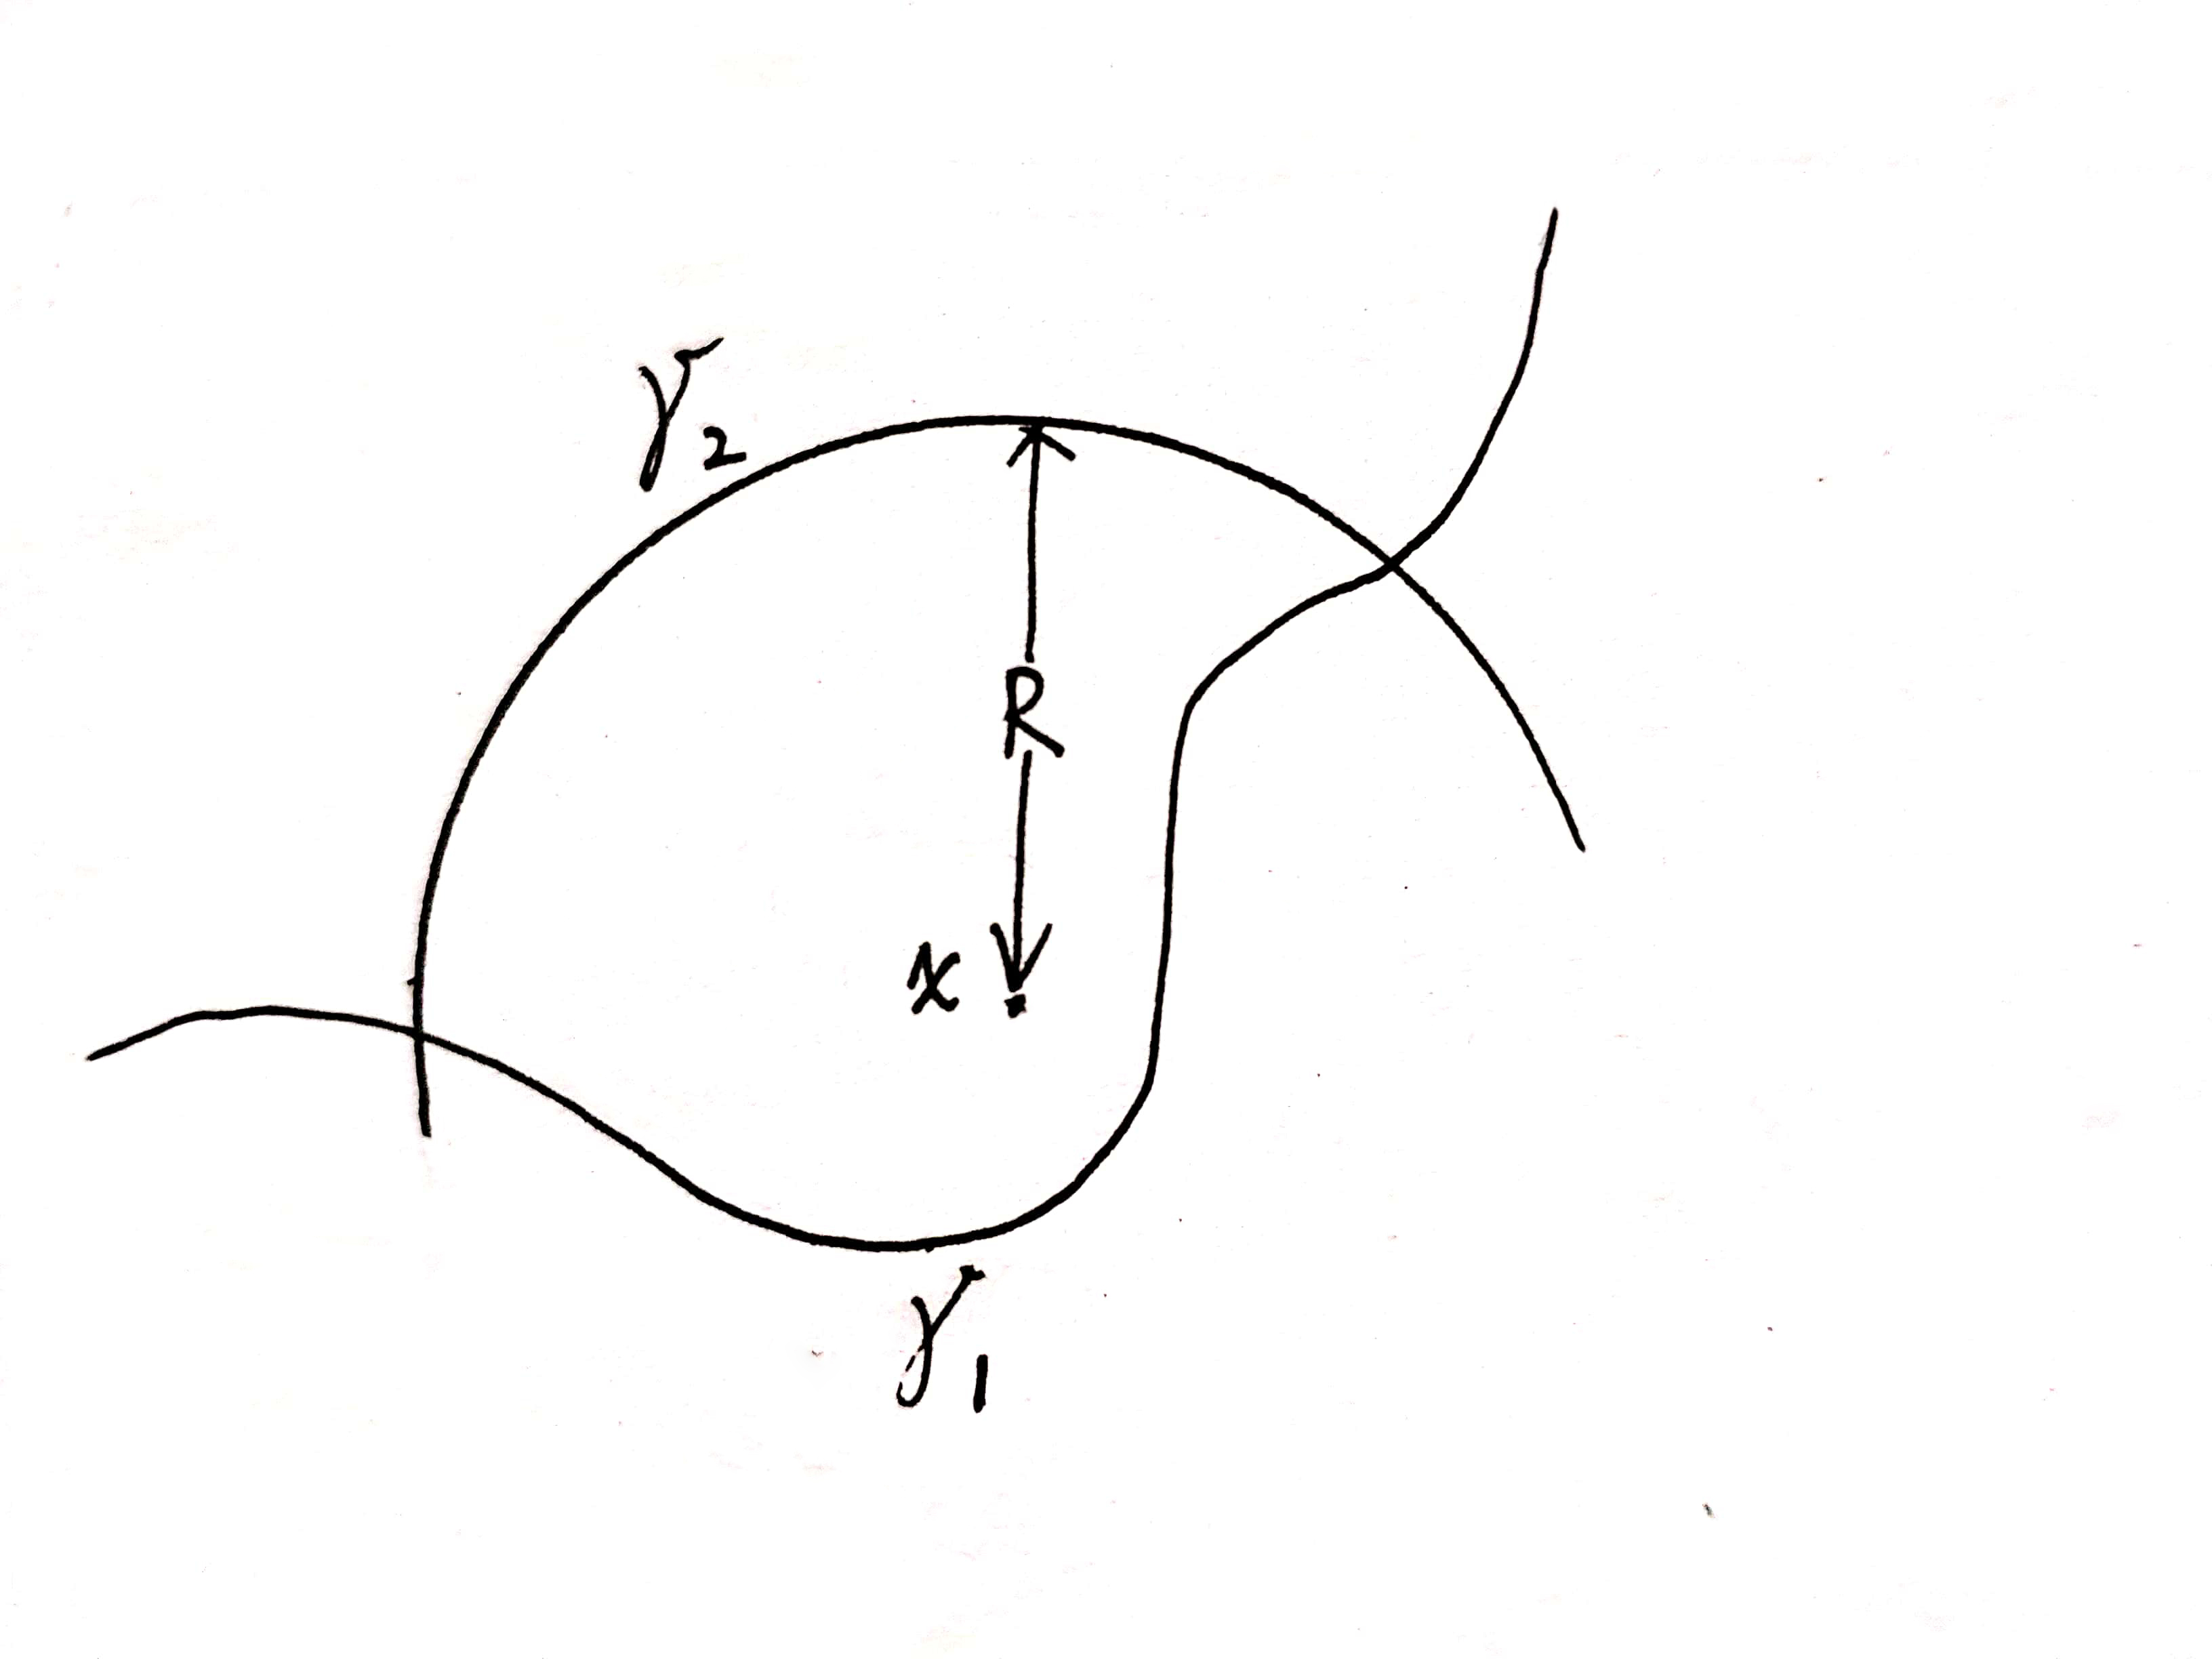
\includegraphics[width=10cm]{PDE1_4_6.jpg}
        \caption{$\Omega_R$}
        \label{pde1_4_6}
    \end{figure}
    
    于是利用Green公式,对每个固定的$R$,我们可以证明
    \begin{align}
    u(x)&= -\int_{\Omega_R} \Gamma(x-y) \Delta u(y) \dy + \int_{\partial \Omega_R} \left(\Gamma(x-y) \frac{\partial u}{\partial \bm{n}_y}(y) -u(y)\frac{\partial \Gamma}{\partial \bm{n}_y}(x,y)   \right) \dS_y \notag \\
    &=-\int_{\Omega_R} \Gamma(x-y) \Delta u(y) \dy + \int_{\gamma_1} \left(\Gamma(x-y) \frac{\partial u}{\partial \bm{n}_y}(y) -u(y)\frac{\partial \Gamma}{\partial \bm{n}_y}(x,y)   \right) \dS_y \notag \\
    &+\int_{\gamma_2} \left(\Gamma(x-y) \frac{\partial u}{\partial \bm{n}_y}(y) -u(y)\frac{\partial \Gamma}{\partial \bm{n}_y}(x,y)   \right) \dS_y. \notag
    \end{align}
    显然我们有$$
    \lim_{R \to \infty}    \Omega_R = \Omega ,\qquad \lim_{R \to \infty} \gamma_1 = \partial \Omega, $$
    关键在于证明$$
    \lim_{R \to \infty}\int_{\gamma_2} \left(\Gamma(x-y) \frac{\partial u}{\partial \bm{n}_y}(y) -u(y)\frac{\partial \Gamma}{\partial \bm{n}_y}(x,y)   \right) \dS_y =0. $$
    $n \ge 3$时,
    \begin{align}
    &\quad \lim_{R \to \infty} \left|\int_{\gamma_2} \left(\Gamma(x-y) \frac{\partial u}{\partial \bm{n}_y}(y) -u(y)\frac{\partial \Gamma}{\partial \bm{n}_y}(x,y)   \right) \dS_y \right| \notag \\
    &\le \lim_{R \to \infty} C(n) R^{n-1} \left( \left| \Gamma(x-y) \frac{\partial u}{\partial \bm{n}_y}(y) \right|+\left|u(y)\frac{\partial \Gamma}{\partial \bm{n}_y}(x,y)   \right| \right) \notag \\
    &\le \lim_{R \to \infty} C(n) R^{n-1} \left( O\left(\frac{1}{R^{n-2}}\right) \cdot o\left(\frac{1}{R}\right) +o(1) \cdot O\left(\frac{1}{R^{n-1}}\right)   \right) \notag \\
    &= \lim_{R \to \infty} C(n) R^{n-1} \left(  o\left(\frac{1}{R^{n-1}}\right) + o\left(\frac{1}{R^{n-1}}\right) \right) \notag \\
    &= 0 \notag
    \end{align}
    {\color{red}{$n=2$时,上面第一项的估计会难以进行,我们认为需要加强衰减性条件,需要$$
            u(x)=o(1),\qquad |\nabla u(x)|=o\left( \frac{1}{|x|\ln|x|} \right), \qquad |x| \to \infty. $$}}
    在新修订的教材上,添加了这样的条件$\exists a,C >0$,使得$$
    |x|^a u(x)+|x|^{1+a} |Du(x)| + |x|^{2+a} |D^2 u(x)| \le C. $$
    如此,我们的证明可以进行下去了.其中二阶导数的控制条件应当是为了使得要证的式子第一项积分有意义.
    
    \subsection{$\S_{1.4}$第7题}
    \kaishu{}验证$n\ge3$维情形下定理1.4.2成立.\\
    
    \songti{}\uuline{解答}:\\
    
    定理1.4.2即
    \begin{equation*}
    u(x)=- \int_{\partial B_1} g(y) \frac{\partial G}{\partial \bm{n}_y}(x,y) \dS_y,\quad x \in B_1
    \end{equation*}
    是调和方程
    \begin{equation*}
    \begin{cases}
    \Delta u =0,&x \in B_1,\\
    u = g, &x \in \partial B_1
    \end{cases}
    \end{equation*}
    的解.
    由Green函数的定义,显然有$\Delta u = 0$.关键在于证明$u$满足边界条件,即证
    \begin{equation*}
    \forall x \in \partial B_1 ,\lim_{x \to x^0}u(x) =g(x^0).
    \end{equation*}
    我们将在本节第10题的解答中给出公式$$
    \frac{\partial G}{\partial \bm{n}_y}=- \frac{1-|x|^2}{w_{n-1}|x-y|^n},\qquad \forall n. $$
    的证明,这里我们直接使用它.
    \begin{align*}
    u(x)-u(x^0)&=\int_{\partial B_1}  \frac{1-|x|^2}{w_{n-1}|x-y|^n} (g(y)-g(x^0))\dS_y\\
    &=\left(\int_{\partial B_1 \cap \{|y-x^0| \le |x-x^0|^{\frac{1}{n+1}}\}}+\int_{\partial B_1 \cap \{|y-x^0| \ge |x-x^0|^{\frac{1}{n+1}}\}}  \right)\frac{1-|x|^2}{w_{n-1}|x-y|^n} (g(y)-g(x^0))\dS_y\\
    &\xlongequal{\Delta}I_1+I_2.
    \end{align*}
    接下来的工作和书上的做法是类似的,不再赘述.
    
    \subsection{$\S_{1.4}$第9题}
    \kaishu{}
    \begin{enumerate}
        \item 求半圆区域上的Dirichlet 问题的Green 函数;
        \item 求$H = \{(x_1, \dots , x_n)|x_{n−1}, x_n > 0\} $上的Dirichlet 问题的Green 函数.
    \end{enumerate}
    
    \songti{}\uuline{解答}:\\
    
    \begin{enumerate}
        \item 圆盘上的Green函数为$$
        \Gamma(x-y)=\frac{1}{2\pi}\ln \frac{1}{|x-y|}. $$
        我们将使用静电源像法解决这个问题.
        \begin{figure}[htbp]
            \centering
            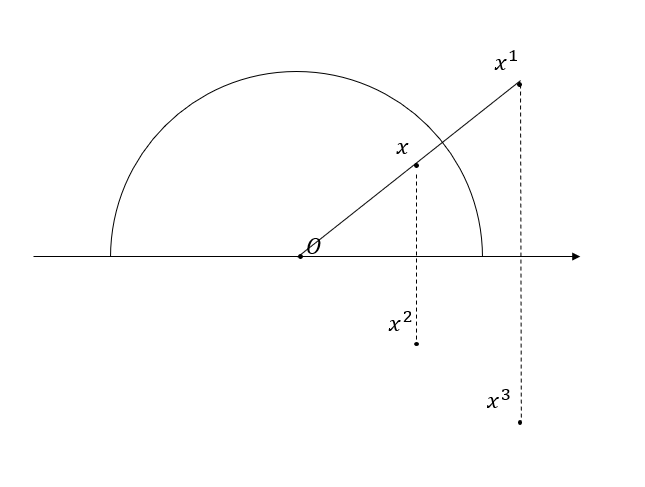
\includegraphics[width=10cm]{PDE1_4_9_1.jpg}
        \end{figure}
        如图,$x^1$是$x$关于圆周的反演点,故$x^1=\frac{R^2}{|x|}x$,在圆周上,应有
        \begin{align*}
        \Gamma(x^1-y)&=\frac{1}{2\pi}\ln \frac{1}{|x^1-y|}\\
        &=\frac{1}{2\pi}\ln \frac{1}{|\frac{R^2}{|x|}x-y|}\\
        &=\frac{1}{2\pi} \left( \ln \frac{1}{|Rx-\frac{|x|}{R}y|}+\ln\frac{|x|}{R} \right)\\
        &\xlongequal{|Rx-\frac{|x|}{R}y|=|x-y|}\Gamma(x-y)+\frac{1}{2\pi}\ln\frac{|x|}{R}
        \end{align*}
        为了平衡直径上的电荷,继续引入$x^2$和$x^3$,分别为$x^2=-x$,$x^3=-x^1=-\frac{R^2}{|x|}x$.与$x^1$类似,我们有
        \begin{align*}
        &\Gamma(x^3-y)=\Gamma(x^2-y)+\frac{1}{2\pi}\ln\frac{|x|}{R} \qquad \text{在圆周上}.\\
        &\begin{cases}
        \Gamma(x-y)&=\Gamma(x^2-y) \\
        \Gamma(x^1-y)&=\Gamma(x^3-y)
        \end{cases}\qquad \text{在直径上}.
        \end{align*}
        为了平衡整个边界上的电势,取$$
        \gamma(x,y)=\Gamma(x^1-y)-\Gamma(x^2-y)+\Gamma(x^3-y). $$
        于是,半圆区域上的Green函数为\begin{align*}
        G(x-y)&=\Gamma(x-y)-\Gamma(x^1-y)+\Gamma(x^2-y)-\Gamma(x^3-y)\\
        &=\frac{1}{2\pi}\ln\frac{|x^1-y||x^3-y|}{|x-y||x^2-y|}.
        \end{align*}
        
        \item 与第1问的做法类似,设$x=(x_1, \dots ,x_{n−1}, x_n)$,则引入三个电荷如下
        \begin{figure}[htbp]
            \centering
            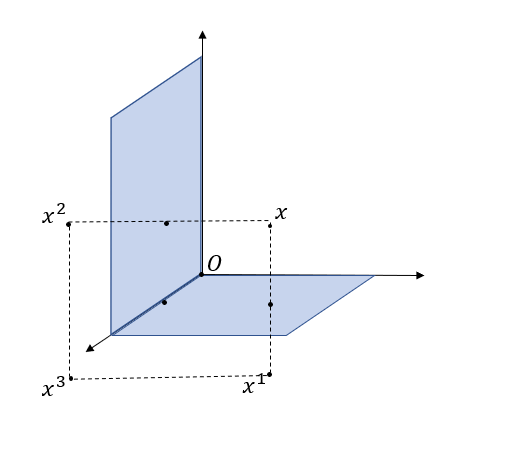
\includegraphics[width=10cm]{PDE1_4_9_2.jpg}
        \end{figure}
        \begin{align*}
        x^1&=(x_1, \dots ,-x_{n−1}, x_n)\\
        x^2&=(x_1, \dots ,x_{n−1}, -x_n)\\
        x^3&=(x_1, \dots ,-x_{n−1},- x_n).
        \end{align*}
        于是,四分之一全空间上的Green函数为
        \begin{align*}
        G(x-y)&=\Gamma(x-y)-\Gamma(x^1-y)+\Gamma(x^2-y)-\Gamma(x^3-y).
        \end{align*}
        具体的表达式与维数有关,此处不再赘述.
    \end{enumerate}
    
    \subsection{$\S_{1.4}$第10题}
    \kaishu{}利用公式(1.54)重新证明单位球上调和函数的Harnack不等式.\\
    
    \songti{}\uuline{解答}:\\
    
    公式(1.54)指的是$$
    u(x)=-\int_{\partial \Omega} u(y) \frac{\partial G}{\partial \bm{n}_y}\dS_y. $$
    应当指出,书上证明Harnack不等式主要使用的是平均值性质,容易看出公式(1.54)形式上也是一种平均性质.\\
    $\Omega=B_1$,不妨$\Omega^{\prime}$取成半径较小的同心球$B_r$.我们首先指出在单位球面上有$$
    \frac{\partial G}{\partial \bm{n}_y}=- \frac{1-|x|^2}{w_{n-1}|x-y|^n},\qquad \forall n. $$
    虽然这个等式只要求个导数就能得到,但为了让这份习题解答更受用户的满意,我们决定稍后补上这个等式的证明.现在\begin{align*}
    u(x)&=-\int_{\partial B_1} u(y) \frac{\partial G}{\partial \bm{n}_y}\dS_y\\
    &=\int_{\partial B_1} u(y) \frac{1-|x|^2}{w_{n-1}|x-y|^n}\dS_y\\
    &\begin{cases}
    \le \frac{1}{(1-r)^n} \frac{1}{w_{n-1}} \int_{\partial B_1} u(y) \dS_y\\
    \ge \frac{1-r^2}{(1+r)^n} \frac{1}{w_{n-1}} \int_{\partial B_1} u(y) \dS_y
    \end{cases},\text{这里用到$x$在球$B_r$里,而$y$在球面$\partial B_1$上.}\\
    &\begin{cases}
    \le \frac{1}{(1-r)^n}  u(0)\\
    \ge \frac{1-r^2}{(1+r)^n}  u(0)
    \end{cases}
    \end{align*}
    接下来的操作和书上的做法是类似的,请读者自行完成.我们接下来将给出单位球面上Green函数的径向导数的公式证明.读者必须注意,虽然维数不同,Green函数的形式略有不同,但它们的径向导数并没有区别,因此我们在这里不对维数$n$进行讨论.\begin{align*}
    \frac{\partial G}{\partial \bm{n}_y}&\xlongequal{\text{单位球面}} \frac{\partial G}{\partial |y|} \\
    &=\frac{\partial G}{\partial y} \cdot \bm{n}_y\\
    &\xlongequal{\text{单位球面}}\frac{\partial G}{\partial y} \cdot y\\
    &=-\frac{1}{w_{n-1}} \left( |x-y|^{-(n-1)}\frac{y-x}{|y-x|}  -\left|\frac{R}{|x|} x -\frac{|x|}{R}y\right|^{-(n-1)} \frac{\frac{|x|}{R}y-\frac{R}{|x|} x}{\left|\frac{|x|}{R}y-\frac{R}{|x|} x\right|}\frac{|x|}{R} \right)\cdot y\\
    &\xlongequal{\text{单位球面}} -\frac{1}{w_{n-1}} \left( |x-y|^{-(n-1)}\frac{y-x}{|y-x|}  -\left|\frac{1}{|x|} x -|x|y\right|^{-(n-1)} \frac{|x|y-\frac{1}{|x|} x}{\left||x|y-\frac{1}{|x|} x\right|}|x| \right)\cdot y \\
    &\xlongequal{|x-y|=\left|\frac{x}{|x|}  -|x|y\right|} -\frac{1}{w_{n-1}|x-y|^n} (y-x-|x|^2 y+x) \cdot y\\
    &\xlongequal{y\cdot y=1}- \frac{1-|x|^2}{w_{n-1}|x-y|^n}.
    \end{align*}
    
    
    
    \subsection{$\S_{1.4}$第11题}
    \kaishu{}
    (1) \textbf{Harnack 第一定理}\quad 设函数序列$\{u_k\} \subset  C(\bar{\Omega}) $为$\Omega$上的调和函数列.若$\{u_k\}$ 在$\partial \Omega$ 上一致收敛, 则它在$\Omega$ 上也一致收敛, 并且极限函数$u $也
    是$\Omega $上的调和函数.\\
    
    (2)\textbf{ Harnack 第二定理}\quad 设$\{u_k\}$为$\Omega$上的一个单调不减的调和函数列.若$\{u_k\}$在$\Omega$中的某点P处收敛, 则它内闭一致收敛于$\Omega$ 上的一个调和函数$u $.\\
    
    \songti{}\uuline{解答}:\\
    
    \uline{\textbf{Harnack 第一定理}}
    
    由于$\{u_k\}$在$\partial \Omega$ 上一致收敛,从而由$Cauchy$收敛原理:
    
    $\forall \varepsilon \ge0,\forall x\in \partial \Omega,\exists N$,只要$m,n\geq N$则有
    $$|u_m(x)-u_n(x)|\leq \varepsilon.$$
    由于$u_m(x),u_n(x)$调和,从而差函数调和,由极值原理:极大值在边界取到,即$\forall y\in \Omega$
    $$|u_m(y)-u_n(y)|\leq|u_m(x)-u_n(x)|\leq \varepsilon.$$
    所以,$u_n(x)$在$\Omega$上,依最大模范数为$Cauchy$列,再由$Cauchy$收敛原理,$u_k$在$\Omega$上一致收敛.
    
    下证极限函数调和.
    
    记$u=lim_{k \to \infty}u_k$,即$u$为极限函数.
    
    由调和函数的平均值不等式知
    $$u_k(x_0)=\frac{1}{|\partial B_R(x_0)|}\int_{\partial B_R(x_0)}u_k(x)\dx,$$
    
    两边同时取$k \to \infty$有
    \begin{align*}
    u(x_0)&=\lim\limits_{k \to \infty}u_k(x_0)\\
    &=\frac{1}{|\partial B_R(x_0)|}\lim\limits_{k \to \infty}\int_{\partial B_R(x_0)}u_k(x)\dx\\
    &\xlongequal{\text{由一致收敛}}\frac{1}{|\partial B_R(x_0)|}\int_{\partial B_R(x_0)}\lim\limits_{k \to \infty}u_k(x)\dx\\
    &=\frac{1}{|\partial B_R(x_0)|}\int_{\partial B_R(x_0)}u(x)\dx.
    \end{align*}
    从而,$u(x)$满足平均值性质,由$\S_{1.4}$第13题知$u(x)$为调和函数.\\
    
    \uline{\textbf{Harnack 第二定理}}
    
    利用$u_n$单调不减,对于非负调和函数$u_n(x)-u_1(x)$应用Harnack不等式
    
    $\forall\Omega'\subset \subset \Omega,\exists C(\Omega',\Omega)$,使得$\forall y\in \overline{\Omega}'$有
    \begin{align*}
    u_n(y)-u_1(y)&\leq C(\Omega',\Omega)(u_n(p)-u_1(p))\\&\leq C(\Omega',\Omega)(u(p)-u_1(p))\\&< \infty.
    \end{align*}
    
    由$n$的任意性,知$u(y)=\lim\limits_{n \to \infty}u_n(y)=\lim\limits_{n \to \infty}(u_n(y)-u_1(y))+u_1(y)<\infty,$
    从而极限函数$u(x)$本身良定义(即点态收敛).
    
    为证$u_n(x)$一致收敛,只需说明:$\forall \varepsilon,\exists N,s.t.\forall x$,当$m,n>N$时有:$|u_n(x)-u_m(x)|<\varepsilon.$
    
    由于$u_n(x)$单调不减,不妨设$m>n$,则$u_m(x)-u_n(x)>0$,由Harnack不等式知$\exists C(\Omega',\Omega) s.t.$
    $$u_m(x)-u_n(x)<(u_m(p)-u_n(p))C(\Omega',\Omega),$$
    
    由于$u_n(x)$在$p$点收敛,可取到$N$,使得:$|u_m(p)-u_n(p)|<\frac{\varepsilon}{C(\Omega',\Omega)}.$从而$|u_m(x)-u_n(x)|<\varepsilon.$至于极限函数$u$的调和性,和Harnack第一定理的证明是类似的.
    
    
    
    \subsection{$\S_{1.4}$第12题}
    \kaishu{}证明Dirichlet 外问题和Dirichlet 问题的等价性. (提示: 利用Kelvin 变换和奇点可去性定理.) 利用该等价性证明有界区域外定义的调和函数若在无穷远
    衰减到0, 则衰减速度至少为$O(\frac{1}{r})$.\\
    
    \songti{}\uuline{解答}:\\
    
    先声明一个观察:Kelvin变换作为对函数的变换具有形式上的对合性.
    
    我们记Kelvin变换为$K$,那么形式上$K^2=Id$,这是因为
    \begin{align*}
    &\qquad K[f](x)=\frac{1}{|x|^{n-2}}f(\frac{x}{|x|^2})\\
    &\Rightarrow f(\frac{x}{|x|^2})=|x|^2 K[f](x)\\
    &\xLongrightarrow{y=\frac{x}{|x|^2}} f(y)=\frac{1}{|y|^{n-2}} K[f](\frac{y}{|y|^2})\\
    &\xLongrightarrow{g=K[f]} K^{-1}[g](y)=\frac{1}{|y|^{n-2}} g(\frac{y}{|y|^2})
    \end{align*}
    定义映射
    \begin{align*}
    \tilde{K}:     \mathbb{R}^n &\rightarrow \mathbb{R}^n\\
    x &\mapsto \frac{x}{|x|^2}
    \end{align*}
    为了方便起见,$\tilde{K}$仍称为Kelvin变换,仍记作$K$,容易验证Kelvin变换作为对点集的映射具有形式上的对合性.
    
    回到原题,我们先证明:\uline{任意一个Dirichlet问题可以导出某个Dirichlet外问题}
    
    不失一般性,我们假设$0\in \Omega$,设$u$是以下Dirichlet问题的解
    $$
    \begin{cases}
    -\Delta u=f & in \quad \Omega\\
    u= g & on  \quad \partial \Omega
    \end{cases} $$
    我们断言,$v=K[u]$是以下Dirichlet外问题的解
    $$
    \begin{cases}
    -\Delta v=K[f] & in \quad K(\Omega)\\
    v= K[g] & on  \quad \partial K(\Omega)\\
    \begin{cases}
    \lim_{x \to \infty} v(x)=0 & n\ge 3\\
    \sup_x |v(x)| < \infty &n=2
    \end{cases}
    \end{cases} $$
    证明: 首先,$v$满足的这一组方程确实是一个Dirichlet外问题,因为$0\in \Omega$,故$K(\Omega)$是一个不含$0$的无界区域.这里我们强调$K(\Omega)$不含$0$只是为了方便,事实上如果$K(\Omega)$含$0$或者$\Omega$不含$0$,无非是将Kelvin变换做一个平移,并不影响这个问题的本质.另一方面
    \begin{align*}
    v(x)&=K[u](x)=\frac{1}{|x|^{n-2}}u(\frac{x}{|x|^2})\\
    &\xlongequal{y=\frac{x}{|x|^2}} |y|^{n-2} u(y)\\
    &\begin{cases}
    \to 0 &n \ge 3\\
    < \infty &n=2
    \end{cases}\qquad x \to \infty.
    \end{align*}
    最后一步得以成立源于$u$的调和性.
    
    再证明,\uline{这个Dirichlet外问题可以导出原来的Dirichlet问题}.
    
    由Kelvin变换的对合性容易得到我们要证的结果,对合性的说明在上文已经详细陈述了.关键在于$u=K^{-1}[v]$在$0$点的定义问题,这由奇点可去性定理可以很容易得到.
    
    我们应当注意,在由Dirichlet问题导出的Dirichlet外问题往回推导Dirichlet问题时,选取的Kelvin变换并不一定要以$0$点为心,但很容易证明这样推导出的Dirichlet问题和原来的Dirichlet问题也是等价的.
    
    \subsection{$\S_{1.4}$第13题}
    \kaishu{}证明满足平均值性质的连续函数一定是调和函数.(提示: 利用Poisson 公式和极值原理的证明思想)\\
    
    \songti{}\uuline{解答}:\\
    
    按照提示,设$u$是满足平均值性质的连续函数,由平均值性质可以推出极值原理,故$u$有极值原理.由Poisson公式,记以$u$的边界值为边界的调和函数为$v$,则$u-v$也满足极值原理,但是在边界上取值恒为0,故$u-v\equiv 0$.
    
    另外,也可以先证明$u\in C^{\infty}$,再将证明平均值性质的过程倒推回去即可.事实上,由调和函数的解析性,$u\in C^{\infty}$是显然的.%todo我们给出另外一种利用卷积证明调和函数$u\in C^{\infty}$的办法.
    
    \section{特征值问题}
    
    \subsection{内容提要}
    \begin{itemize}
        \item 特征值问题是下两章分离变量法的基础.
        \item Sturm-Liouville定理.\\
        \kaishu{}
        考虑1D上$\Omega=(0, L)$的特征值问题:
        $$\begin{cases}
        -u''(x) = \lambda u(x), \quad , x\in(0, L),\\
        -\alpha_1u'(0) + \beta_1u(0)=0,\\
        \alpha_2u'(L) + \beta_2u(L) = 0,
        \end{cases}$$
        其中$\alpha_i\geq0, \beta_i\geq0, \alpha_i + \beta_i \neq 0, i=1,2$.则有以下结论:
        \songti{}
        \begin{enumerate}
            \item 所有的特征值都是非负的,且构成趋于$+\infty$的单调递增序列,即
            $$0\leq \lambda_1\leq \lambda_2 \leq \dots\leq \lambda_k\leq\dots\rightarrow\infty,$$
            且$\lambda_1=0 \Leftrightarrow \beta_1=\beta_2=0$.
            \item 存在一列特征函数$\{u_k\}_{k=1}^\infty\in C^\infty(\overline{\Omega})$,对应特征值$\lambda_k$,构成$L^2(0, L)$上的一组{\bf 完备标准正交基}. 且$\forall f\in L^2(0, L),$其可以表示为
            $$f(x) = \sum_{i=1}^\infty a_ku_k(x).$$其在$L^2(0, L)$意义下收敛.
            \item 若$f\in C^2([0, L])$且满足相应的边界条件,则上式绝对一致收敛.
        \end{enumerate}
        \item 一般区域上的Poincar\'{e}不等式:\\
        对于任意$u\in C^1(\overline{\Omega}), \bm{u|_{\partial\Omega}=0}$,
        $$ \int_\Omega |\nabla u|^2 \dx \geq \frac1{D^2}\int_\Omega u^2 \dx,$$
        其中$D := \sup_{x,y\in\Omega}|x-y|$为直径.且第一特征值$\lambda_1$为使得不等式成立的最佳常数,有$\lambda_1 \geq \frac1{D^2}$.
    \end{itemize}
    
    
    \subsection{$\S_{1.5}$第1题}
    \kaishu{}求解如下带Neumann边值的Laplace算子特征值问题:
    \begin{equation*}
    \begin{cases}
    -u^{''}(x) = \lambda u(x), \quad x \in (0,\pi),\\
    u(0) = u^{'}(\pi) = 0.
    \end{cases}
    \end{equation*}\\
    
    \songti{}\uuline{解答}:\\
    
    方程的通解为:
    \begin{equation*}
    \begin{cases}
    A\cos\sqrt{\lambda}x + B \sin \sqrt{\lambda}x, &\lambda >0,\\
    Ax+B , &\lambda = 0,\\
    Ae^{\sqrt{-\lambda}x}+ Be^{-\sqrt{-\lambda}x}, &\lambda <0.
    \end{cases}
    \end{equation*}
    考虑边界条件,易得$\lambda>0$且$\lambda_k = (k-\frac12)^2,k\ge1$.于是方程的解为
    \begin{equation*}
    u_k = \frac{\sin(k-\frac12)x}{k-\frac12},k\ge 1 .
    \end{equation*}
    
    \subsection{$\S_{1.5}$第2题}
    \kaishu{}证明Sturm-Liouville定理,即定理1.5.1.\\
    
    \songti{}\uuline{解答}:\\
    
    应用紧算子的谱理论即可.
    
    \subsection{$\S_{1.5}$第3题}
    \kaishu{}证明:(1.69)中的特征函数$\{u_k\}_{k=1}^{\infty}$构成$L^2(\Omega)$的一组完备的标准正交基,这里$\Omega=(0,a)\times (0,b) \subset \mathbb{R}^2$.\\
    
    \songti{}\uuline{解答}:\\
    
    标准性和正交性都是显然的,只要证完备性.由一维Fourier级数理论,易知$L^2(0,a)$中的函数能被三角多项式$v_k = \sqrt{\frac2a}\sin\frac{k\pi}{a}x$一致逼近.读者有兴趣的话可以通过奇延拓的方法证明这个问题.
    
    又由实变函数理论,$L^2$空间中的函数可以被阶梯函数一致逼近,于是
    \begin{equation*}
    \forall g \in L^2(\Omega),\quad \exists \{c_{ij}\},\{A_{ij}\} ,s.t. \quad g = \sum_{i,j=1}^{\infty}c_{ij}1_{A_{ij}}.
    \end{equation*}
    其中$c_{ij}$是常数,$A_{ij}$是小矩形可测区域.而
    \begin{equation*}
    1_{A_{ij}} = 1_{A_{i}} 1_{A_{j}}.
    \end{equation*}
    其中$A_{i},A_{j}$分别是$(0,a),(0,b)$上的可测集.于是$1_{A_{i}},1_{A_{j}}$可以分别被三角多项式$$\sqrt{\frac2a}\sin\frac{i\pi}{a}x,\sqrt{\frac2b}\sin\frac{j\pi}{b}x$$一致逼近,这就得到了我们要的结论.
    
    \chapter{热方程}
    \section{方程的物理背景和定解问题}
    
    \subsection{内容提要}
    \begin{itemize}
        \item 这一节研究什么?
        \begin{enumerate}
            \item 提出热方程的定解问题(初边值问题, Cauchy问题)
            \item 使用分离变量法求解初边值问题
            \item 使用Fourier变换求解Cauchy问题
            \item 解的性质(极值原理, 梯度估计, Harnack不等式, 古代解的性质, 解的时间衰减性, 能量方法),进一步得到解的唯一性,稳定性
        \end{enumerate}
    \end{itemize}
    
    \section{分离变量法和初边值问题解的存在性}
    \subsection{内容提要}
    \begin{itemize}
        \item 分离变量法的使用方法.
        \begin{enumerate}
            \item 寻找可变量分离的,且满足{\bf 齐次}边界条件的特解,在1D的情况下由于齐次边界条件,我们可以得到可列个符合条件的特征值和特征向量(特解).
            \item 将特解线性组合得到通解,利用初始条件求解待定的系数,其在1D下即为Fourier级数的求解.
            \item 检验解符合定解问题.
        \end{enumerate}
    \end{itemize}
    \subsection{$\S_{2.2}$第1题}
    \kaishu{}利用分离变量法求解初边值问题
    \begin{equation*}
    \begin{cases}
    \partial_t u = a^2\partial_x^2 u, &(t,x) \in (0,+\infty) \times I,\\
    u(0,x)=\varphi(x), &x \in I,\\
    \partial_xu(t,0) = \partial_x(t,L)=0,&t \in (0,+\infty).
    \end{cases}
    \end{equation*}
    其中$\varphi$满足相容性条件$\varphi^{\prime}(0)=\varphi^{\prime}(L)=0$,常数$a \in \mathbb{R}^{+}$.\\
    
    \songti{}\uuline{解答}:\\
    
    设$u(t,x) = T(t)X(x)$,代入方程后可以得到
    \begin{equation*}
    T^{\prime}(t)X(x)-a^2T(t)X^{\prime\prime}(x) =0.
    \end{equation*}
    考虑非平凡的情形,则有
    \begin{equation*}
    \frac{T^{\prime}(t)}{T(t)} = a^2 \frac{X^{\prime\prime}(x)}{X(x)}.
    \end{equation*}
    左边是$t$的函数,右边是$x$的函数,故它只能是常数,因此$\exists \lambda \in \mathbb{R}$,使得
    \begin{equation*}
    \frac{T^{\prime}(t)}{T(t)} = -\lambda=a^2 \frac{X^{\prime\prime}(x)}{X(x)}.
    \end{equation*}
    类似书上的做法,很容易得到$\lambda$应当取正值,此时
    \begin{align*}
    T(t)&=T_0 e^{-\lambda t},\\
    X(x) &=C_1 \sin(\frac{\sqrt{\lambda}}{a}x)+C_2 \cos(\frac{\sqrt{\lambda}}{a}x).
    \end{align*}
    考虑到边界条件,我们可以解得特解为
    \begin{equation*}
    u(t,x) = C_{\lambda} e^{-\lambda t}\cos(\frac{\sqrt{\lambda}}{a}x),
    \end{equation*}
    其中$\lambda = \left(\frac{ak\pi}{L}\right)^2 $.记$\varphi(x)$的Fourier展开为
    \begin{equation*}
    \varphi(x) = \sum_{k=1}^{\infty} a_k \cos(\frac{k\pi}{L}x),
    \end{equation*}
    那么我们得到了分离变量的解
    \begin{equation*}
    u(t,x) = \sum_{k=1}^{\infty} a_k e^{-\lambda_k t}\cos(\frac{k\pi}{L}x).
    \end{equation*}
    
    \subsection{$\S_{2.2}$第4题}
    \kaishu{}利用第一章第五节中贝塞尔函数的性质,求解二维单位圆$B_1 \subset \mathbb{R}^2$内热方程的初边值问题
    \begin{equation*}
    \begin{cases}
    \partial_t u - \Delta u = 0, &(t,x) \in (0,+\infty) \times B_1,\\
    u(0,x) = \varphi(x),&x \in B_1,\\
    u = 0, &(t,x) \in (0,+\infty) \times \partial B_1.
    \end{cases}
    \end{equation*}
    其中$\varphi \in C^2(\overline{B_1})$满足$\left.\varphi \right|_{\partial B_1} = 0$.\\
    
    \songti{}\uuline{解答}:\\
    
    考虑分离变量形式的解$u(t,x) = T(t) X(x)$,代入方程后得到
    \begin{equation*}
    \frac{T^{'}(t)}{T(t)} = \frac{\Delta X}{X(x)} = -\lambda.
    \end{equation*}
    \begin{itemize}
        \item $\lambda = 0$,此时$X(x)$是一个调和函数,由边界条件及调和函数的极值原理,易知$u\equiv 0$.
        \item $\lambda < 0$,此时如果$X(x)$不恒为0,则不妨设$X(x)$在$x_0$处取得正的最大值,则$X(x)$在$x_0$处的Hessian矩阵半负定.但是此时$tr(H(x_0)) = \Delta X(x_0) = -\lambda X(x_0) > 0$,矛盾!
        \item $\lambda >0$,此时由贝塞尔函数的性质,
        \begin{equation*}
        X_{n,l}(x) = C_{n,l}J_n(\sqrt{\lambda_{n,l}}r).
        \end{equation*}
        我们这里的贝塞尔函数都是标准化的,它们又是完备的,于是可以令初值$\varphi$关于贝塞尔函数展开成Fourier级数,
        \begin{equation*}
        \varphi(x) = \sum_{n,l=1}^{\infty} a_{n,l}J_n(\sqrt{\lambda_{n,l}}r).
        \end{equation*}
        因此分离变量形式的解为
        \begin{equation*}
        u(t,x) = \sum_{n,l=1}^{\infty} a_{n,l} e^{-\lambda_{n,l} t}J_n(\sqrt{\lambda_{n,l}}r).
        \end{equation*}
    \end{itemize}
    
    \subsection{$\S_{2.2}$第5题}
    \kaishu{}求解非齐次热方程的初边值问题
    \begin{equation*}
    \begin{cases}
    \partial_t u - \partial^2_x u = \cos x, &(t,x) \in (0,+\infty) \times (0,2\pi),\\
    u(0,x) = \cos2x,&x \in(0,2\pi),\\
    u_x(t,0) = u_x(t,2\pi) =0,&(t,x) \in (0,+\infty).
    \end{cases}
    \end{equation*}\\
    
    \songti{}\uuline{解答}:\\
    
    使用分离变量法,易知特征函数列为$\{\cos kx\}_{k=0}^{\infty}$,直接使用公式,
    \begin{align*}
    u(t,x) &= \int_0^te^{-\tau} \cos x \d\tau + e^{-4t}\cos2x\\
    &=(1-e^{-t})\cos x + e^{-4t}\cos2x.
    \end{align*}
    
    \subsection{$\S_{2.2}$第6题}
    \kaishu{}证明$t>0$时(2.14)式是$C^2$一致收敛的.\\
    
    \songti{}\uuline{解答}:\\
    
    只要证明了原级数一致收敛,便可以利用逐项求导性质证明其$C^2$一致收敛.
    \begin{align*}
    |u(t,x)| & =| \sum_{k=1}^{\infty} a_k e^{-\lambda_k t}\sin\sqrt{\lambda_k}x|\\
    &\le \sum_{k=1}^{\infty} |a_k e^{-\lambda_k t}\sin\sqrt{\lambda_k}x|\\
    &\le \sum_{k=1}^{\infty}| a_k |\\
    &< \infty.
    \end{align*}
    最后一步是因为$\varphi \in C^2(I) \cap C^1(\overline{I})$,故其Fourier系数收敛.
    
    \section{Fourier变换和Cauchy问题解的存在性}
    \subsection{内容提要}
    \begin{itemize}
        \item 1D中的Fourier变换及其性质.\\
        \begin{enumerate}
            \item Fourier变换: 若$f\in L^1(\mathbb{R}_x),$则其Fouirer变换:
            $$\widehat{f}(\cosy) = \int_\mathbb{R} f(x)e^{-i\cosy x}\dx$$
            Fourier逆变换: 若$\hat{g}\in L^1(\mathbb{R}_\cosy),$则其Fouirer逆变换:
            $$g(x) = \frac1{2\pi}\int_\mathbb R \widehat g(\cosy)e^{i\cosy x}\d\cosy.$$
            \item Fourier变换是线性的.
            \item Fourier变换可以把导数弄下来.\\
            若$f, f'\in L^1(\mathbb R_x)$,则
            $$\widehat{(f')} = i\cosy \widehat f.$$
            若$f(x), xf(x)\in L^1(\mathbb R_x)$,则
            $$\left( \widehat f\right)'  = -i \widehat{(xf)}.$$
            \item Fourier变换可以把卷积变成乘积.\\
            卷积: 对于$f_1, f_2\in L^1(\mathbb R)$,
            $$f_1 * f_2 = \int_\mathbb{R} f_1(x-y)f_2(y)\dy = \int_\mathbb{R}f_1(y)f_2(x-y)\dy.$$
            则有
            \begin{align*}
            \widehat{(f_1 * f_2)} &= \widehat{f_1} \cdot \widehat{f_2}\\
            \mathcal{F}^{-1}(f_1\cdot f_2) &= \mathcal{F}^{-1}(f_1) * \mathcal{F}^{-1}(f_2)
            \end{align*}
            \item Fourier变换还有很多重要而有趣的性质,此处懒得继续列出.高维的Fourier有类似的性质.
        \end{enumerate}
        \item 由n维的Cauchy问题得到的热核:
        $$H_t(x) = \mathcal{F}^{-1}[e^{-|\cdot|^2t}](x) = \frac1{(4\pi t)^{\frac n2}}e^{-\frac{|x|^2}{4t}}.$$
        及其性质的应用:若$\varphi\in L^p(\mathbb R^n), 1\leq p\leq+\infty$,记$P_t\varphi(x)= \varphi * H_t(x)$,则
        \begin{enumerate}
            \item $P_t\varphi$是热方程$\partial_t u = \Delta u$的解(验证了Cauchy问题解的存在性,利用热核的衰减性质可以交换求导和积分次序),
            \item 对于任意$t>0$,有$\|P_t\varphi\|_{L^p} \leq \|\varphi\|_{L^p}$(利用Young不等式,$\|H_t\|_{L^1} = 1$,但这不意味着解是唯一的!),
            \item 对于任意$t,s>0$,有$P_{t+s}\varphi = P_t(P_s\varphi)$,
            \item 如果$p<+\infty$,则$\lim_{t\rightarrow 0_+} \|P_t\varphi -\varphi\|_{L^p(\mathbb{R}^n)} = 0$.(验证了Cauchy问题解的存在性)
        \end{enumerate}
        \item 热方程解的无穷传播速度.由Cauchy问题解的表达式得到,即使初值是有紧支集的,也会在下一刻支集变为全空间.
    \end{itemize}
    
    
    \subsection{$\S_{2.3}$第5题}
    \kaishu{}利用一维热方程解的表达式(2.24)证明:若$\varphi \in C(\mathbb{R}) \cap L^{\infty}(\mathbb{R})$,则当$t>0$时,解$u(t,x)$关于$x$是解析函数.并进一步证明Weierstrass逼近定理:若$f(x)$是有界闭区间$[a,b]$上的连续函数,则它可以被多项式序列一致逼近.(提示:取
    \begin{equation*}
    \varphi(x) =
    \begin{cases}
    f(a),&x\ge a ,\\
    f(x), &a\le x \le b,\\
    f(b), &x \ge b,
    \end{cases}
    \end{equation*}
    利用解$u$关于$x$的解析性,并取$t \to 0_{+}$.) \\
    
    \songti{}\uuline{解答}:\\
    
    表达式(2.24)即为
    \begin{equation*}
    u(t,x) = \frac{1}{2\sqrt{\pi t}} \int_{\mathbb{R}} \varphi(y) e^{-\frac{(x-y)^2}{4t}}\dy.
    \end{equation*}
    这个公式我们是建议读者背下来的,包括其高维形式.从这个表达式中,由指数函数的衰减性及解析性,易见$u(t,x)$关于$x$是解析的.后面一个问题由热核的恒等逼近性质就可以得到,不再赘述.
    
    
    \subsection{$\S_{2.3}$第9题}
    \kaishu{}验证若$f(t,x)$关于时间$t$一阶可导,关于空间$x$三阶连续可导,且各阶导数有界,$\varphi \in C(\mathbb{R}^n) \cap L^{\infty}(\mathbb{R}^n)$,则(2.29)式给出了Cauchy问题(2.28)的解. \\
    
    \songti{}\uuline{解答}:\\
    
    (2.29)式即
    \begin{align*}
    u(t,x) &=\frac{1}{(4\pi t)^{\frac{n}{2}}} \int_{\mathbb{R}^n}\varphi(y) e^{-\frac{|x-y|^2}{4t}}\dy\\
    &+ \int_0^t  \int_{\mathbb{R}^n}\varphi(y)\frac{1}{(4\pi (t-\tau))^{\frac{n}{2}}} f(\tau,y)e^{-\frac{|x-y|^2}{4(t-\tau)}}\dy \d\tau\\
    &\xlongequal{\Delta}I_1+ I_2.
    \end{align*}
    (2.28)即
    \begin{equation*}
    \begin{cases}
    \partial_t u - \Delta u = f(t,x), &(t,x) \in (0,+\infty) \times \mathbb{R}^n,\\
    u(0,x) = \varphi(x), &x\in \mathbb{R}^n.
    \end{cases}
    \end{equation*}
    我们已经知道,$I_1$是方程
    \begin{equation*}
    \begin{cases}
    \partial_t u - \Delta u = 0, &(t,x) \in (0,+\infty) \times \mathbb{R}^n,\\
    u(0,x) = \varphi(x), &x\in \mathbb{R}^n.
    \end{cases}
    \end{equation*}
    的解,由叠加原理,我们只要证明$I_2$是方程
    \begin{equation*}
    \begin{cases}
    \partial_t u - \Delta u = f(t,x), &(t,x) \in (0,+\infty) \times \mathbb{R}^n,\\
    u(0,x) = 0, &x\in \mathbb{R}^n.
    \end{cases}
    \end{equation*}
    的解.显然有
    \begin{equation*}
    \lim\limits_{t \to 0_{+}} I_2 = 0.
    \end{equation*}
    形式上,$I_2 = \int_0^t \varphi\ast H(t-\tau,x)\d\tau$.因此
    \begin{align*}
    (\partial_t - \Delta)I_2 &=
    \lim\limits_{\tau \to t} \varphi\ast H(t-\tau,x) \\
    &+ \int_0^t \varphi\ast (\partial_t - \Delta)H(t-\tau,x)\d\tau\\
    &\xlongequal{\text{热核恒等逼近性质}}f(t,x).
    \end{align*}
    
    \subsection{$\S_{2.3}$第11题}
    \kaishu{}对于$n\ge 3$,对于任意$x,y \in \mathbb{R}^n,x\ne y,$
    \begin{equation*}
    \int_0^{\infty}H(t,x-y)\dt = \Gamma(x-y) = \frac{1}{(n-2)\omega_{n-1}|x-y|^{n-2}}.
    \end{equation*}     \\
    
    \songti{}\uuline{解答}:\\
    
    不妨将$x-y$视作整体,记为$x$,
    \begin{align*}
    \int_0^{\infty}H(t,x)\dt &=\int_0^{\infty}\frac{1}{(4\pi t)^{\frac{n}{2}}}e^{-\frac{|x|^2}{4t}}\dt\\
    &\xlongequal{z = \frac{|x|^2}{4t}}\int_{\infty}^0 \frac{1}{(4\pi \frac{|x|^2}{4z})^{\frac{n}{2}}} e^{-z} \frac{|x|^2}{-4z^2}\dz\\
    &=\int_0^{\infty} \frac{1}{4\pi^{\frac{n}{2}}|x|^{n-2}}e^{-z} z^{\frac{n}{2}-2}\dz\\
    &=\frac{\Gamma(\frac{n}{2}-1)}{4\pi^{\frac{n}{2}}|x|^{n-2}}\\
    &=\frac{\Gamma(\frac{n}{2})}{2(n-2)\pi^{\frac{n}{2}}|x|^{n-2}}.
    \end{align*}
    而$n$维球体的体积为
    \begin{equation*}
    V_n = \frac{\pi^{\frac{n}{2}}}{\Gamma(\frac{n}{2}+1)}R^n.
    \end{equation*}
    所以
    \begin{align*}
    \omega_{n-1}&= \frac{n\pi^{\frac{n}{2}}}{\Gamma(\frac{n}{2}+1)}\\
    &=\frac{n\pi^{\frac{n}{2}}}{\frac{n}{2}\Gamma(\frac{n}{2})}
    =\frac{2\pi^{\frac{n}{2}}}{\Gamma(\frac{n}{2})}.
    \end{align*}
    代入即可.
    
    \uline{另外一种方法利用Fourier变换}:\\
    
    令$u=x-y, u\neq0$,则对$\int_0^\infty H(t, u)\dt$做Fourier变换得:
    $$\int_0^\infty \widehat H(t, u)\dt = \int_0^\infty e^{-t|\cosy|^2} \dt = \frac1{|\cosy|^2}.$$
    则对$\Gamma(u)$做Fourier变换,有$$\widehat{\Gamma}(\cosy) = \int_{\mathbb R^n}\Gamma(u)e^{-i\cosy u}du.$$
    但后续验证变换后的结果相等(即积分上式)较难,需要用到复变函数的知识,此处从略.
    
    \section{热方程解的极值原理}
    \subsection{$\S_{2.4}$第1题}
    \kaishu{}假设热方程正解的梯度估计(2.32)在$R=1$时成立,证明对于任意$R>0$,(2.32)成立. \\
    
    \songti{}\uuline{解答}:\\
    
    设u是$(0,T]\times B_R$上热方程$\partial_t u =\Delta u$的正解,构造辅助函数$v(\tilde{t},\tilde{x})$为
    \begin{equation*}
    v(\tilde{t},\tilde{x}) = u(R^2 \tilde{t},R\tilde{x}).
    \end{equation*}
    易见$v$满足热方程$\partial_{\tilde{t}} v =\Delta_{\tilde{x}} v,(\tilde{t},\tilde{x})\in (0,\frac{T}{R^2}]\times B_1$.
    那么,有$R=1$时的梯度估计
    \begin{equation*}
    \frac{|\nabla_{\tilde{x}}v|^2}{v^2}-\alpha \frac{\partial_{\tilde{t}}v}{v} \le \frac{n\alpha^2}{2\tilde{t}}+C\alpha^2(1+\frac{\alpha^2}{\alpha-1}).
    \end{equation*}
    作尺度变换
    \begin{equation}
    t = R^2 \tilde{t},\quad x = R \tilde{x}.
    \end{equation}
    那么
    \begin{align*}
    \frac{\nabla_{\tilde{x}}u|^2}{u^2} &= \frac{R^2|\nabla_{x}u|^2}{u^2},\\
    \frac{\partial_{\tilde{t}}u}{u} &=
    \frac{R^2\partial_{t}u}{u}.
    \end{align*}
    所以我们得到
    \begin{equation*}
    \frac{R^2|\nabla_{x}u|^2}{u^2} - \alpha\frac{R^2\partial_{t}u}{u} \le \frac{n\alpha^2}{2\frac{t}{R^2}}+C\alpha^2(1+\frac{\alpha^2}{\alpha-1}).
    \end{equation*}
    即
    \begin{equation*}
    \frac{|\nabla_{x}u|^2}{u^2} - \alpha\frac{\partial_{t}u}{u} \le \frac{n\alpha^2}{2t}+\frac{C\alpha^2}{R^2}(1+\frac{\alpha^2}{\alpha-1}).
    \end{equation*}
    
    \subsection{$\S_{2.4}$第2题}
    \kaishu{}构造截断函数$\eta$满足(2.37).     \\
    
    \songti{}\uuline{解答}:\\
    
    类似$\S_{1.3}$第4题,我们构造函数$\tilde{\varphi} \in C_c^{\infty}(\mathbb{R})$,满足
    \begin{equation*}
    \tilde{\varphi}=
    \begin{cases}
    1 & |x| \le \frac12,\\
    0 & |x| \ge 1.
    \end{cases}
    \end{equation*}
    易见有
    \begin{equation*}
    \exists c >0 ,\quad |\nabla \tilde{\varphi}|\le \frac{c}{2}, \quad |\Delta \tilde{\varphi}| \le \frac{c}{2}.
    \end{equation*}
    取$\varphi(x) = \tilde{\varphi}(R|x|)$.则
    \begin{equation*}
    \varphi(x)\in C_c^{\infty}(\mathbb{R}^n),\quad
    \exists c >0 ,\quad |\nabla \varphi|\le \frac{c}{2R}, \quad |\Delta \varphi| \le \frac{c}{2R^2}.
    \end{equation*}
    再取$\eta(x) = \varphi(x)^2$.则
    \begin{align*}
    &\eta(x)\in C_c^{\infty}(\mathbb{R}^n),\\
    &\exists c >0 ,\quad |\nabla \eta|= 2\varphi |\nabla \varphi|\le  \frac{c}{R}\eta^{\frac12}, \\
    &|\Delta \eta| = 2|\nabla \varphi|^2 + 2\varphi \nabla \varphi \ge -\frac{c}{R^2}.
    \end{align*}
    
    \subsection{$\S_{2.4}$第3题}
    \kaishu{}对于任意$\alpha>1$    ,证明(2.32)成立. \\
    
    \songti{}\uuline{解答}:\\
    
    我们应当重新叙述一遍定理内容.
    
    设$u$是$(0,T]\times B_R$上热方程$\partial_t u = \Delta u$的正解,$\alpha>1$,对于任意$(t,x) \in (0,T]\times B_{\frac{R}{2}}$,成立
    \begin{equation*}
    \frac{|\nabla u|^2}{u^2} - \alpha \frac{\partial_t u}{u}
    \le \frac{n \alpha^2}{2t} + \frac{C\alpha^2}{R^2}(1+\frac{\alpha^2}{\alpha-1}).
    \end{equation*}
    
    同样我们可以假设$R=1$来证明它.
    
    记$F = t(|\nabla f|^2 - \alpha \partial_t f)$,其中$f=\ln u$,所以有
    \begin{equation*}
    \partial_t f = \Delta f + |\nabla f|^2.
    \end{equation*}
    因此,
    \begin{equation*}
    \Delta f =- \frac{F}{\alpha t} - \frac{\alpha-1}{\alpha} |\nabla f|^2.
    \end{equation*}
    对$\nabla^2f$使用Bochner不等式,得
    \begin{align*}
    \Delta F &\ge 2t \left[ \frac{1}{n} \left(\frac{F}{\alpha t} + \frac{\alpha-1}{\alpha} |\nabla f|^2\right)^2 - \left\langle\nabla f,\nabla\left(\frac{F}{\alpha t} + \frac{\alpha-1}{\alpha} |\nabla f|^2\right)^2\right\rangle +\right. \\
    &\ \quad \left. 2\partial_t\left(\frac{F}{\alpha t} + \frac{\alpha-1}{\alpha} |\nabla f|^2\right) \right]\\
    &\ge \frac{2F^2}{n\alpha^2 t} + \frac{4(\alpha-1)}{n\alpha^2}|\nabla f|^2F-\frac{2}{\alpha}\langle\nabla f, \nabla F \rangle -\frac{2F}{\alpha t}+\\
    &\ \quad 2t \left\langle\nabla f,\nabla\left(-\frac{\alpha-1}{\alpha}|\nabla f|^2 + \frac{2\alpha-1}{\alpha}\partial_t f\right)\right\rangle\\
    &=\frac{2F^2}{n\alpha^2 t} +\frac{4(\alpha-1)}{n\alpha^2}|\nabla f|^2F-2\left\langle\nabla f,\nabla F\right\rangle-\frac{F}{t}+\partial_t f.
    \end{align*}
    同样,我们要求截断函数$\eta\in C^{\infty}_c(B_R),0\le \eta \le 1$,在$B_{\frac{R}{2}}$上恒为1,且有
    \begin{equation*}
    |\nabla \eta|(x) \le \frac{c}{R}\eta^{\frac12},\quad \Delta\eta(x) \ge -\frac{c}{R^2}.
    \end{equation*}
    设$(t_0,x_0)$是$\eta F$的最大值点,不妨$\eta F(t_0,x_0)>0$,$(t_0,x_0)$是抛物区域的内点.那么有估计
    \begin{align*}
    -(\partial_t-\Delta)(\eta F) &=\Delta\eta F+2\langle\nabla \eta,\nabla f\rangle-\eta(\partial_t-\Delta)F\\
    &\ge -cF +2\langle\nabla f,\nabla F\rangle+\eta\left(\frac{2F^2}{n\alpha^2 t} + \frac{4(\alpha-1)}{n\alpha^2}|\nabla f|^2 F-2\langle\nabla f,\nabla F\rangle-\frac{F}{t} \right).
    \end{align*}
    在$(t_0,x_0)$处,$\eta(x_0)>0,\nabla F = \frac{\nabla(\eta F)}{\eta}-\frac{\nabla \eta}{\eta} F $,因此
    \begin{align*}
    -(\partial_t-\Delta)(\eta F)(t_0,x_0) &\ge -cF +\frac{2}{\eta} \langle\nabla \eta,\nabla (\eta F)\rangle-2\frac{|\nabla \eta|^2}{\eta}F +\frac{2\eta F^2}{n\alpha^2t_0} + \frac{4(\alpha-1)}{n\alpha^2}|\nabla f|^2\eta F\\
    &-2\langle\nabla f,\nabla(\eta F)\rangle+2\langle\nabla f,\nabla\eta\rangle F-\frac{\eta F}{t_0}.
    \end{align*}
    由于$(t_0,x_0)$是$\eta F$的最大值点,因此$\nabla(\eta F)(t_0,x_0)=0,\Delta(\eta F)(t_0,x_0)\le0,\partial_t(\eta F)(t_0,x_0)\ge 0$,又
    $\frac{|\nabla \eta|^2}{\eta}\le c $,所以
    \begin{align*}
    0&\ge -cF+\frac{2\eta F^2}{n\alpha^2t_0} + \frac{4(\alpha-1)}{n\alpha^2}|\nabla f|^2\eta F+2\langle\nabla f,\nabla\eta\rangle F-\frac{\eta F}{t_0}.
    \end{align*}
    利用$\eta$的性质,我们可以得到上式其中两项的估计
    \begin{align*}
    \frac{4(\alpha-1)}{n\alpha^2}|\nabla f|^2\eta F+2\langle\nabla f,\nabla\eta\rangle F&\ge \frac{4(\alpha-1)}{n\alpha^2}|\nabla f \eta^{\frac12}|^2 F-2\eta|\nabla f||\nabla \eta|F\\
    &\ge \frac{4(\alpha-1)}{n\alpha^2}|\nabla f \eta^{\frac12}|^2 F-2c|\nabla f\eta^{\frac12}|F\\
    &\ge -\frac{C\alpha^2}{\alpha-1}F.
    \end{align*}
    代回,得到
    \begin{equation*}
    0\ge -c(1+\frac{\alpha^2}{\alpha-1})F+\frac{2\eta F^2}{n\alpha^2t_0}-\frac{\eta F}{t_0}.
    \end{equation*}
    则
    \begin{align*}
    \eta F(t_0,x_0) &\le \frac{n\alpha^2 t_0}{2}\left(\frac{\eta}{t_0}+c(1+\frac{\alpha^2}{\alpha-1})\right)\\
    &\le \frac{n\alpha^2}{2}+Ct_0 \alpha^2(1+\frac{\alpha^2}{\alpha-1}).
    \end{align*}
    在$B_{\frac{R}{2}}$上$\eta$恒为1,两端除以$T$,再将$t_0$放大到$T$即可.
    \subsection{$\S_{2.4}$第4题}
    \kaishu{}证明(2.44)成立.     \\
    
    \songti{}\uuline{解答}:\\
    
    (2.44)即
    \begin{equation*}
    |u_0^{(k)}(t)| \le \frac{k!}{(ct)^k}e^{-\frac{1}{2t^a}},\quad \forall t >0,k\in \mathbb{N}.
    \end{equation*}
    其中
    \begin{equation*}
    u_0(t) =
    \begin{cases}
    e^{-\frac{1}{t^a}}, &t>0,\\
    0,&t\le 0.
    \end{cases}
    \end{equation*}
    注意到$t>0$时,$u_0(t)$是实解析的,因此我们将$t$复化,利用Cauchy积分公式来证明.
    
    取围道$\gamma$为以$t$为圆心,半径$r=ct$的圆,$c$满足
    \begin{equation*}
    Re(z^{-a}) > \frac12 (Re(t))^{-a},\quad \forall z \in \gamma.
    \end{equation*}
    应当注意,$c$足够小时,上式总能成立,因此这样的$c$是能取到的.
    因此
    \begin{align*}
    |u_0^{(k)}(t)|&\le\sup\limits_{t\in \gamma} |u_0(t)|\left|\frac{k!}{(2\pi i)(ct)^k}\right|\\
    &\le \frac{k!}{(2\pi)(ct)^k}e^{-\frac{1}{2t^a}}\\
    &\le \frac{k!}{(ct)^k}e^{-\frac{1}{2t^a}}.
    \end{align*}
    %--------------------------------------------------------------------
    
    
    \section{能量方法和解的唯一性}
    \subsection{$\S_{2.5}$第4题}
    \kaishu{}对具光滑边界的有界区域$\Omega$,若在$\Omega$上传导热量的介质的传热效果是不均匀的,且在各方向上效果不同,我们可以得到变系数的热方程
    \begin{equation*}
    \partial_t u - div(A(x) \nabla u) = \partial_t u - \sum_{i,j=1}^n \partial_{x_i}(a_{ij}(x)\partial_{x_j}u)=0.
    \end{equation*}
    其中$A(x) = (a_{ij}(x))_{i,j=1}^n$是关于$x$充分光滑的矩阵函数,满足对任意给定的$x$,$A(x)$为正定矩阵.当$A(x) =I_n$时,即为我们处理过的常系数热方程.请使用能量方法,证明其初边值问题解的唯一性.
    \begin{equation*}
    \begin{cases}
    \partial_t u - div(A(x) \nabla u) = f(t,x), &(t,x) \in (0,+\infty) \times \Omega,\\
    u(0,x) = \varphi(x),&x \in \Omega,\\
    u(t,x) = g(t,x), &(t,x) \in (0,+\infty) \times \partial \Omega.
    \end{cases}
    \end{equation*}
    其中$\varphi$与$g$满足一定的相容性条件.\\
    
    \songti{}\uuline{解答}:\\
    
    设$u_1,u_2$是方程的两个解,记$w = u_1-u_2$,则
    \begin{equation*}
    \begin{cases}
    \partial_t w - div(A(x) \nabla w) = 0, &(t,x) \in (0,+\infty) \times \Omega,\\
    w(0,x) = 0,&x \in \Omega,\\
    w(t,x) = 0, &(t,x) \in (0,+\infty) \times \partial \Omega.
    \end{cases}
    \end{equation*}
    以$w$作为乘子进行全空间积分,
    \begin{align*}
    0&=\int_{\Omega} w\partial_t w -w div(A(x) \nabla u) \dx\\
    &=\frac12 \frac{\d}{\dt}\int_{\Omega} w^2\dx - \left(\int_{\partial \Omega} wA(x) \frac{\partial w}{\partial \bm{n}}\dS - \int_{\Omega}\nabla w^T A(x) \nabla w \dx \right)\\
    &=\frac12 \frac{\d}{\dt}\int_{\Omega} w^2\dx + \int_{\Omega}\nabla w^T A(x) \nabla w \dx.
    \end{align*}
    记$e(t) = \frac12\int_{\Omega}w^2(t,x) \dx$,  对上式0到$t$积分,即得
    \begin{equation*}
    e(t) + \int_0^t\int_{\Omega}\nabla w^T A(x) \nabla w \dx \d\tau = e(0) = 0.
    \end{equation*}
    又$A(x)$正定,故左端第二项非负,又$e(t)$非负,那么只能
    \begin{equation*}
    e(t) \equiv 0.
    \end{equation*}
    于是$w\equiv0$,这就证明了唯一性.
    
    
    
    \chapter{波动方程}
    
    由于助教同时出了一版习题解答,故此章节(大)部分解答请参考该版本.
    
    \section{方程的物理背景和定解问题}
    
    
    \subsection{$\S_{3.1}$第3题}
    \kaishu{}
    
    1) 假设$\bm E = (E_1, E_2, E_3)$和$\bm B = (B_1, B_2, B_3)$满足Maxwell方程组
    $$ \begin{cases}
    \partial_t \bm E = \curl \bm B,\\
    \partial_t \bm B = -\curl \bm E,\\
    \text{\bf div } \bm E = \text{\bf div } \bm B = 0.
    \end{cases}$$
    证明$E_i, B_i (i=1,2,3)$满足波动方程$\partial_t^2u-\Delta u = 0$.
    
    2)设$\bm u = (u_1, u_2, u_3)$满足线性弹性力学方程组
    $$\partial_t^2\bm u -\mu\Delta \bm u -(\lambda + \mu)\nabla(\text{\bf div }\bm u) = 0,$$
    证明$v := \text{\bf div }\bm u$和$w:=\curl \bm u$满足波动方程,且其波速不同.
    
    \songti{}\uuline{解答}:\\
    
    请参考助教的习题解答.
    
    
    \subsection{$\S_{3.1}$第4题}
    \kaishu{}
    
    试通过合适的自变量变换将方程
    $$\partial_t^2 u - 3\partial_{tx}u - 4\partial_x^2 u = 0,$$
    化为标准的波动方程形式.
    
    \songti{}\uuline{解答}:\\
    
    请参考助教的习题解答.
    
    \section{波动方程的Cauchy问题}
    
    
    \subsection{$\S_{3.2}$第2题}
    \kaishu{}
    
    试证明当$f\in C^2(\mathbb R_+ \times \mathbb R^n)$时,形式解
    $$u(t,x) = \int_0^t S(t-\tau) f(\tau , x)\d\tau, \quad (t,x)\in \mathbb R_+\times \mathbb R^n$$是非齐次波动方程Cauchy问题
    $$\begin{cases}
    \partial_t^2 u -\Delta u = f, & (t,x)\in \mathbb R_+\times \mathbb R^n,\\
    u(0, x) = \partial_t u(0, x) = 0, & x \in \mathbb R^n
    \end{cases}$$
    的解.
    
    \songti{}\uuline{解答}:\\
    
        要验证的是,表达式
    \begin{equation*}
    u(t,x) = \int_0^t S(t-\tau)f(\tau,x)\d\tau
    \end{equation*}
    满足三个性质:
    \begin{enumerate}
        \item $\lim\limits_{t\to 0} u(t,x) = 0,$
        \item $\lim\limits_{t\to 0} \partial_t u(t,x) = 0,$
        \item $\partial_t^2u(t,x) = f(t,x) + \Delta u(t,x).$
    \end{enumerate}
    
    接下来我们来一一证明它们.记$w(t,x;\tau)$是方程
    \begin{equation*}
    \begin{cases}
    \partial_t^2w-\Delta w =0,&(t,x) \in (\tau,+\infty)\times \mathbb{R}^n,\\
    w(\tau,x) = 0,\partial_t w(\tau,x) = f(\tau,x) ,&x \in \mathbb{R}^n.
    \end{cases}
    \end{equation*}
    的解.那么形式上有
    \begin{equation*}
    w(t,x,\tau) = S(t-\tau)f(\tau,x).
    \end{equation*}
    \begin{enumerate}
        \item 显然.
        \item 
        \begin{align*}
        \lim\limits_{t\to 0} \partial_t u(t,x)& = \lim\limits_{t\to 0}\lim\limits_{\tau\to t}w(t,x;\tau)+\lim\limits_{t\to 0} \int_0^t\partial_tw(t,x;\tau)\d\tau\\
        &=\lim\limits_{t\to 0}w(t,x;t) + \lim\limits_{t\to 0} \int_0^t\partial_tw(t,x;\tau)\d\tau=0.
        \end{align*}
        事实上
        \begin{equation*}
        \lim\limits_{t\to 0}w(t,x;t) = w(t,x;t) = 0.
        \end{equation*}
        因此这一项在求二阶导数时不再列出.
        \item
        \begin{align*}
        \partial_t^2u(t,x) &=\left.\partial_t w(t,x;\tau)\right|_{\tau=t} + \int_0^t\partial_t^2w(t,x;\tau)\d\tau\\
        & = f(t,x) + \int_0^t\Delta w(t,x;\tau)\d\tau\\
        & = f(t,x) + \Delta u(t,x).
        \end{align*}
    \end{enumerate}
    
    
    
    
    
    \subsection{$\S_{3.2}$第4题}
    \kaishu{}
    
    试用降维法导出弦振动方程解的d'Alembert公式.
    
    \songti{}\uuline{解答}:\\
    
    请参考助教的习题解答.
    
    
    
    \subsection{$\S_{3.2}$第7题}
    \kaishu{}
    
    求解Cauchy问题
    $$\begin{cases}
    \partial_t^2 u - \partial_x^2u + 2k\partial_t u + k^2 u = 0 , & (t,x)\in \mathbb R_+\times \mathbb R,\\
    u(0, x) = \varphi(x), \partial_t u(0, x) = 0, & x \in \mathbb R.
    \end{cases}$$
    其中$k\in \mathbb R$为常数.
    
    \songti{}\uuline{解答}:\\
    
    请参考助教的习题解答.
    
    
    
    \subsection{$\S_{3.2}$第8题}
    \kaishu{}
    
    求解半无界问题
    $$\begin{cases}
    \partial_t^2 u - \partial_x^2u + \partial_x u - \partial_t u = 0, & (t,x)\in \mathbb R_+\times \mathbb R_+,\\
    u(0, x) = \varphi(x), \partial_t u(0, x) = 0, & x \in [0, +\infty),\\
    u(t, 0) = 0, & t \in [0, +\infty).
    \end{cases}$$
    并思考该问题是否能用奇延拓法求解.
    
    \songti{}\uuline{解答}:\\
    
    请参考助教的习题解答.
    
    
    
    \subsection{$\S_{3.2}$第9题}
    \kaishu{}
    
    考虑KdV方程
    $$\partial_t u + 6u \partial_x u + \partial_x^3 u = 0, \quad (t,x)\in \mathbb R_+\times \mathbb R,$$
    试求该方程的一个具有$u(t, x) = \Phi(x-ct)$形式的特解.其中函数$\Phi$满足
    $\lim_{|x|\rightarrow \infty}\Phi(x) = 0, \lim_{|x|\rightarrow \infty}\Phi'(x) = 0, \lim_{|x|\rightarrow \infty}\Phi''(x) = 0.$
    
    \songti{}\uuline{解答}:\\
    
    请参考助教的习题解答.
    
    
    
    \subsection{$\S_{3.2}$第10题}
    \kaishu{}
    
    求解半无界弦振动方程的初边值问题
    $$\begin{cases}
    \partial_t^2 u - a^2 \partial_x^2 u = 0, & (t,x)\in \mathbb R_+\times \mathbb R_+,\\
    u(0, x) = \varphi(x), \partial_t u(0, x) = \psi(x), & x \in \mathbb R_+,\\
    u(t, 0) = c u_x(t, 0), & t\in \mathbb R_+.
    \end{cases}$$
    其中$a,c$为常数,$a\neq c$,初值$\varphi,\psi \in C^2(\mathbb R_+),$分别在$x=0$的某个邻域内恒为0.
    
    \songti{}\uuline{解答}:\\
    
    请参考助教的习题解答.
    
    
    
    \subsection{$\S_{3.2}$第11题}
    \kaishu{}
    
    \songti{}\uuline{解答}:\\
    
    请参考助教的习题解答.
    
    \section{波的传播与衰减}
    
    
    \subsection{$\S_{3.3}$第2题}
    \kaishu{}
    
    证明: 对二维波动方程,若初值$(\varphi, \psi)$光滑且有紧支集,则其Cauchy问题的解在$t\rightarrow+\infty$时, 以$t^{-frac12}$速度一致趋于0.
    
    \songti{}\uuline{解答}:\\
    
    请参考助教的习题解答.
    
    
    
    \subsection{$\S_{3.3}$第3题}
    \kaishu{}
    
    考虑三维Cauchy问题,假定$\varphi \equiv 0 , \psi\in C^\infty(\mathbb R^3)$,
    且$(1+|x|^4)|\phi(x)|$在全空间有界.证明: 存在一个不依赖于$\psi$的常数$C>0$,使得
    $$|u(t,x)| \leq \frac{C\|(1+|x|^4)|\psi(x)|\|_{C^0}}{1+t^{\frac13}}, \quad \forall t \geq 1, |x|=t.$$
    思考一下,当$1+|x|^4$换成$1+|x|^k$,其中$k>2$是常数时,能得到关于时间怎样的衰减.
    
    \songti{}\uuline{解答}:\\
    
    请参考助教的习题解答.
    
    \section{波动方程的初边值问题解的存在性}
    
    
    
    \subsection{$\S_{3.4}$第4题}
    \kaishu{}
    
    考虑初边值问题
    $$\begin{cases}
    \partial_t^2 u = 4\partial_x^2 u, & (t, x) \in \mathbb R_+ \times (0, 1),\\
    u(0, x) = 4\sin^3\pi x, \partial_t u(0, x) = 30x(1-x), & x\in [0, 1],\\
    u(t, 0) = u(t, 1) = 0, & t\in \mathbb R_+.
    \end{cases}$$
    1)求$h(\frac13)$,其中$h(t):= \int_0^1 [u_t^2 + 4u_x^2]\dx$;\\
    2)求$u(2,x)$.
    
    
    \songti{}\uuline{解答}:\\
    
    请参考助教的习题解答.
    
    \section{能量方法和解的唯一性与稳定性}
    
    
    
    
    \subsection{$\S_{3.5}$第3题}
    \kaishu{}
    
    设$u\in C^2([0, T]\times \bar\Omega)$为初边值问题
    $$\begin{cases}
    \partial_t^2u - \Delta u  = f(t,x), & (t, x)  \in\Omega_t,\\
    u(0, x) = \varphi(x), \partial_t u(0,x) = \psi(x), & x \in Omega,\\
    u(t,x) = 0, & (t,x)\in (0, T )\times\partial\Omega.
    \end{cases}$$
    的解,试说明关于解的$L^2$能量估计成立:
    $$\int_\Omega u^2(t,x)\dx \leq C (\|\varphi\|^2_{L^2(\Omega)} +  \|\nabla \varphi\|^2_{L^2(\Omega)} + \|\psi\|^2_{L^2(\Omega)} + \|f\|^2_{L^2(\Omega_T)}), \quad \forall t \in [0, T],$$
    其中$C = C(T) > 0 $为常数.
    
    \songti{}\uuline{解答}:\\
    
    \begin{align*}
    &\quad u(t,x) = u(0,x) + \int_0^t \partial_t u \dt\\
    &\Rightarrow u^2(t,x) \le 2u^2(0,x)+2\left(\int_0^t \partial_t u \dt\right)^2.
    \end{align*}
    又
    \begin{align*}
    \left(\int_0^t \partial_t u \dt\right)^2 &\le t\int_0^t \left(\partial_t u\right)^2 \dt\\
    &\le 2TE(t)\\
    &\le C\left(\|\psi\|^2_{L^2(\Omega)} + \|\nabla \varphi\|^2_{L^2(\Omega)}  + \|f\|^2_{L^2(\Omega_T)} \right).
    \end{align*}
    于是
    \begin{align*}
    \int_{\Omega}u^2(t,x)\dx &\le \int_{\Omega}u^2(0,x)\dx + C\left(\|\psi\|^2_{L^2(\Omega)} + \|\nabla \varphi\|^2_{L^2(\Omega)}  + \|f\|^2_{L^2(\Omega_T)} \right)\\
    &\le C\left(\|\varphi\|^2_{L^2(\Omega)}+\|\psi\|^2_{L^2(\Omega)} + \|\nabla \varphi\|^2_{L^2(\Omega)}  + \|f\|^2_{L^2(\Omega_T)} \right).
    \end{align*}
    
    %
    %
    %
    %
    %
    %
    %
    %
    %
    %
    \iffalse%解题模板
    
    \subsection{$\S_{2.4}$第1题}
    \kaishu{}        \\
    
    \songti{}\uuline{解答}:\\
    
    \fi
    
\end{document}